\documentclass[format=sigconf,anonymous=true,review=true]{acmart}

\usepackage[dvipsnames]{xcolor}

%% Configurações de metadados da ACM (Obrigatórios)
% \setcopyright{none}
% \settopmatter{printacmref=false}
% \renewcommand\ACMconfid{Review}

\usepackage{booktabs}
\usepackage{subcaption}
\usepackage{tikz}
\usetikzlibrary{shapes.geometric, arrows.meta, positioning, calc, fit, backgrounds}
\usepackage{multirow}
\usepackage{graphicx}

% Configuração para fontes Type 42 
\pdfinclusioncopyfonts=1

\begin{document}

% \title{Simultaneous Multi-objective Optimization of Offshore Wind Farm Layout, Substation Placement, and Cable Grouping}

\title{Multi-objective Genetic Algorithm Optimization of Offshore Wind Farm Layout, Substation Placement, and Cable Grouping}


\author{Anonymized for Review}
\affiliation{
  \institution{Anonymized Institution}
  \city{Anonymized City}
  \country{Anonymized Country}
}

\renewcommand{\shortauthors}{Anonymized et al.}

\begin{abstract}
Offshore wind farm (OWF) design involves tightly coupled aerodynamic and electrical decisions that are often optimized sequentially, potentially leading to sub-optimal trade-offs. This paper presents a comparative study of three evolutionary optimization paradigms for OWF co-design: (i) a single-phase NSGA-II optimizing energy production and cabling cost from the outset, (ii) a sequential approach optimizing turbine layout prior to electrical infrastructure design, and (iii) a hierarchical two-phase strategy that combines layout-focused exploration with subsequent multi-objective refinement. All methods are evaluated on a commonly adopted OWF toy problem with increasing farm sizes. Results show that the proposed two-phase strategy consistently achieves higher-quality Pareto fronts, balancing net annual energy production and cabling cost more effectively than purely sequential or single-phase approaches, while maintaining reasonable computational overhead. The study highlights the impact of problem decomposition and optimization strategy on solution quality in real-world evolutionary design problems.
\end{abstract}

%% CCS Concepts - Gerado para Computação Evolutiva e Engenharia
% \begin{CCSXML}
% <ccs2012>
%  <concept>
%   <concept_id>10010147.10010257.10010293.10010290</concept_id>
%   <concept_desc>Computing methodologies~Genetic algorithms</concept_desc>
%   <concept_significance>500</concept_significance>
%  </concept>
%  <concept>
%   <concept_id>10010583.10010717.10010721.10010725</concept_id>
%   <concept_desc>Hardware~Resource optimization</concept_desc>
%   <concept_significance>300</concept_significance>
%  </concept>
% </ccs2012>
% \end{CCSXML}

% \ccsdesc[500]{Computing methodologies~Genetic algorithms}
% \ccsdesc[300]{Hardware~Resource optimization}

\keywords{Offshore Wind Farms, Multi-objective Optimization, Cable Routing, NSGA-II, Substation Placement}

\maketitle

\section{Introduction}

Offshore wind power is a key component of the global energy transition, benefiting from high and stable wind resources and increasing deployment worldwide. Despite its technological maturity, offshore wind farms remain capital intensive, with subsea electrical infrastructure accounting for approximately 11\% to 15\% of total project costs \cite{Alencar2026Flexible, IRENA2024Costs}. A central challenge arises from the strong coupling between turbine layout and electrical collection system design: turbine repositioning to mitigate wake losses directly affects cable length, Joule losses, and routing feasibility.

Most Wind Farm Layout Optimization (WFLO) studies primarily focus on maximizing Annual Energy Production (AEP) through wake mitigation \cite{Silva2025Layout, Baker2019Best}. While this approach yields aerodynamically efficient layouts, it may lead to economically unfavorable solutions once electrical infrastructure is considered. Conversely, recent advances in the Wind Farm Cable Routing Problem (WFCRP) typically assume fixed turbine and substation locations, addressing electrical optimization as a secondary and decoupled task \cite{Alencar2026Flexible, Machado2024Hybrid}. As a result, the interaction between aerodynamic layout decisions and electrical design choices remains insufficiently explored.

Integrated optimization frameworks have emerged to address this limitation, demonstrating that simultaneous consideration of layout and electrical infrastructure can reduce overall project costs \cite{Wang2019Integrated, Jin2025Integrated}. However, two gaps persist in the literature. First, most approaches treat the number of collector strings as fixed, limiting topological flexibility. Second, the transition between rapid layout exploration and detailed electrical refinement is often handled in a disjointed manner, increasing sensitivity to local optima and computational burden.

This work extends the modular genetic algorithm framework proposed in \cite{Silva2025Layout, Silva2025b} toward an integrated multi-objective co-design setting. The offshore wind farm design problem is formulated with $2n+3$ decision variables, where $n$ denotes the number of turbines, capturing turbine positions, substation location, and cable topology. The framework explicitly explores the trade-off between maximizing Net AEP—accounting for wake and electrical losses—and minimizing total cabling cost.

Rather than proposing a new evolutionary algorithm, this paper presents a comparative analysis of three evolutionary optimization paradigms: (i) a single-phase NSGA-II optimizing layout and electrical variables simultaneously \cite{Deb2002NSGA2}, (ii) a sequential two-phase strategy in which layout optimization precedes electrical design, and (iii) a hierarchical two-phase approach that combines layout-focused exploration with subsequent multi-objective refinement. The main contributions of this work are summarized as follows:

\begin{itemize}
    \item A two-phase hierarchical optimization strategy that leverages mono-objective layout exploration to guide subsequent multi-objective co-optimization.
    \item A phase-bridging population initialization mechanism that seeds high-quality layouts while diversifying substation locations to preserve exploration.
    \item A deterministic angular sector grouping strategy that enforces planar, non-overlapping cable strings without the need for geometric repair heuristics.
\end{itemize}


\section{Related Work}

The optimization of offshore wind farms (OWFs) has evolved from simple geometric layouts to high-dimensional, multidisciplinary design problems involving aerodynamic, electrical, and economic objectives. This section reviews prior work on wind farm layout optimization, cable routing, and integrated co-design approaches, with emphasis on evolutionary and meta-heuristic methods.

\subsection{Wind Farm Layout Optimization (WFLO)}
Wind Farm Layout Optimization (WFLO) aims to mitigate wake-induced energy losses, which significantly degrade the performance of downstream turbines. Classical analytical wake models, such as the Jensen model \cite{Jensen1983Wake, Katic1986Simple} and the Gaussian formulations proposed by Bastankhah and Porté-Agel \cite{Bastankhah2014Gaussian, Bastankhah2016Gaussian}, are widely adopted due to their computational efficiency and suitability for optimization loops. These models are commonly embedded in Genetic Algorithms and hybrid meta-heuristics to address the non-convex turbine placement problem \cite{Haupt2004, Qureshi2023Hybrid}. Benchmark-driven studies, such as those based on the IEA Task~37 framework \cite{Baker2019Best}, have further standardized comparative evaluations of WFLO methods. However, most WFLO approaches focus exclusively on maximizing gross AEP, neglecting electrical infrastructure and leading to layouts that may be energetically optimal but economically inefficient \cite{Silva2025Layout}.

\subsection{Wind Farm Cable Routing Problem (WFCRP)}
The Wind Farm Cable Routing Problem (WFCRP) is an NP-hard combinatorial problem that seeks to minimize the cost of connecting turbines to offshore substations while respecting electrical and geometric constraints. Early solutions relied on Mixed-Integer Linear Programming (MILP) formulations \cite{Fischetti2015MILP} or heuristic algorithms such as the Esau--Williams method \cite{Jiangyi2025Topology}. A central difficulty in WFCRP is the enforcement of non-crossing cable layouts, which has motivated the use of geometric repair heuristics, detours, or delayed embedding strategies \cite{Alencar2026Flexible, Ye2023Path}. Recent work has explored multi-agent and swarm-based meta-heuristics to improve scalability \cite{Machado2024Hybrid, Yuan2025ACO}, as well as topology-driven designs such as ring or hybrid networks \cite{Shen2023Ring}. Nevertheless, most WFCRP studies assume fixed turbine and substation locations, treating routing as a secondary optimization step.

\subsection{Integrated Co-Design and Substation Placement}
Integrated optimization of turbine layout and electrical infrastructure has gained increasing attention as a means to reduce overall project costs. Several studies show that optimizing substation location jointly with cable routing yields measurable cost reductions compared to sequential approaches \cite{Moon2015Optimal, Jin2019PowerLoss, Jin2025Integrated}. Other works incorporate cable sizing, electrical losses, and cost models directly into the optimization loop \cite{Wang2019Integrated, Nakhai2023Electrical}. Despite these advances, two limitations remain prevalent in the literature. First, the number of collector strings is typically predefined rather than treated as a decision variable. Second, few studies systematically compare different evolutionary optimization strategies and problem decompositions for the fully coupled layout–infrastructure problem, particularly in terms of convergence behavior and Pareto front diversity.

\section{Methodology}
\label{sec:methodology}

\begin{figure*}[htbp]
  \centering
  \resizebox{\textwidth}{!}{ 
    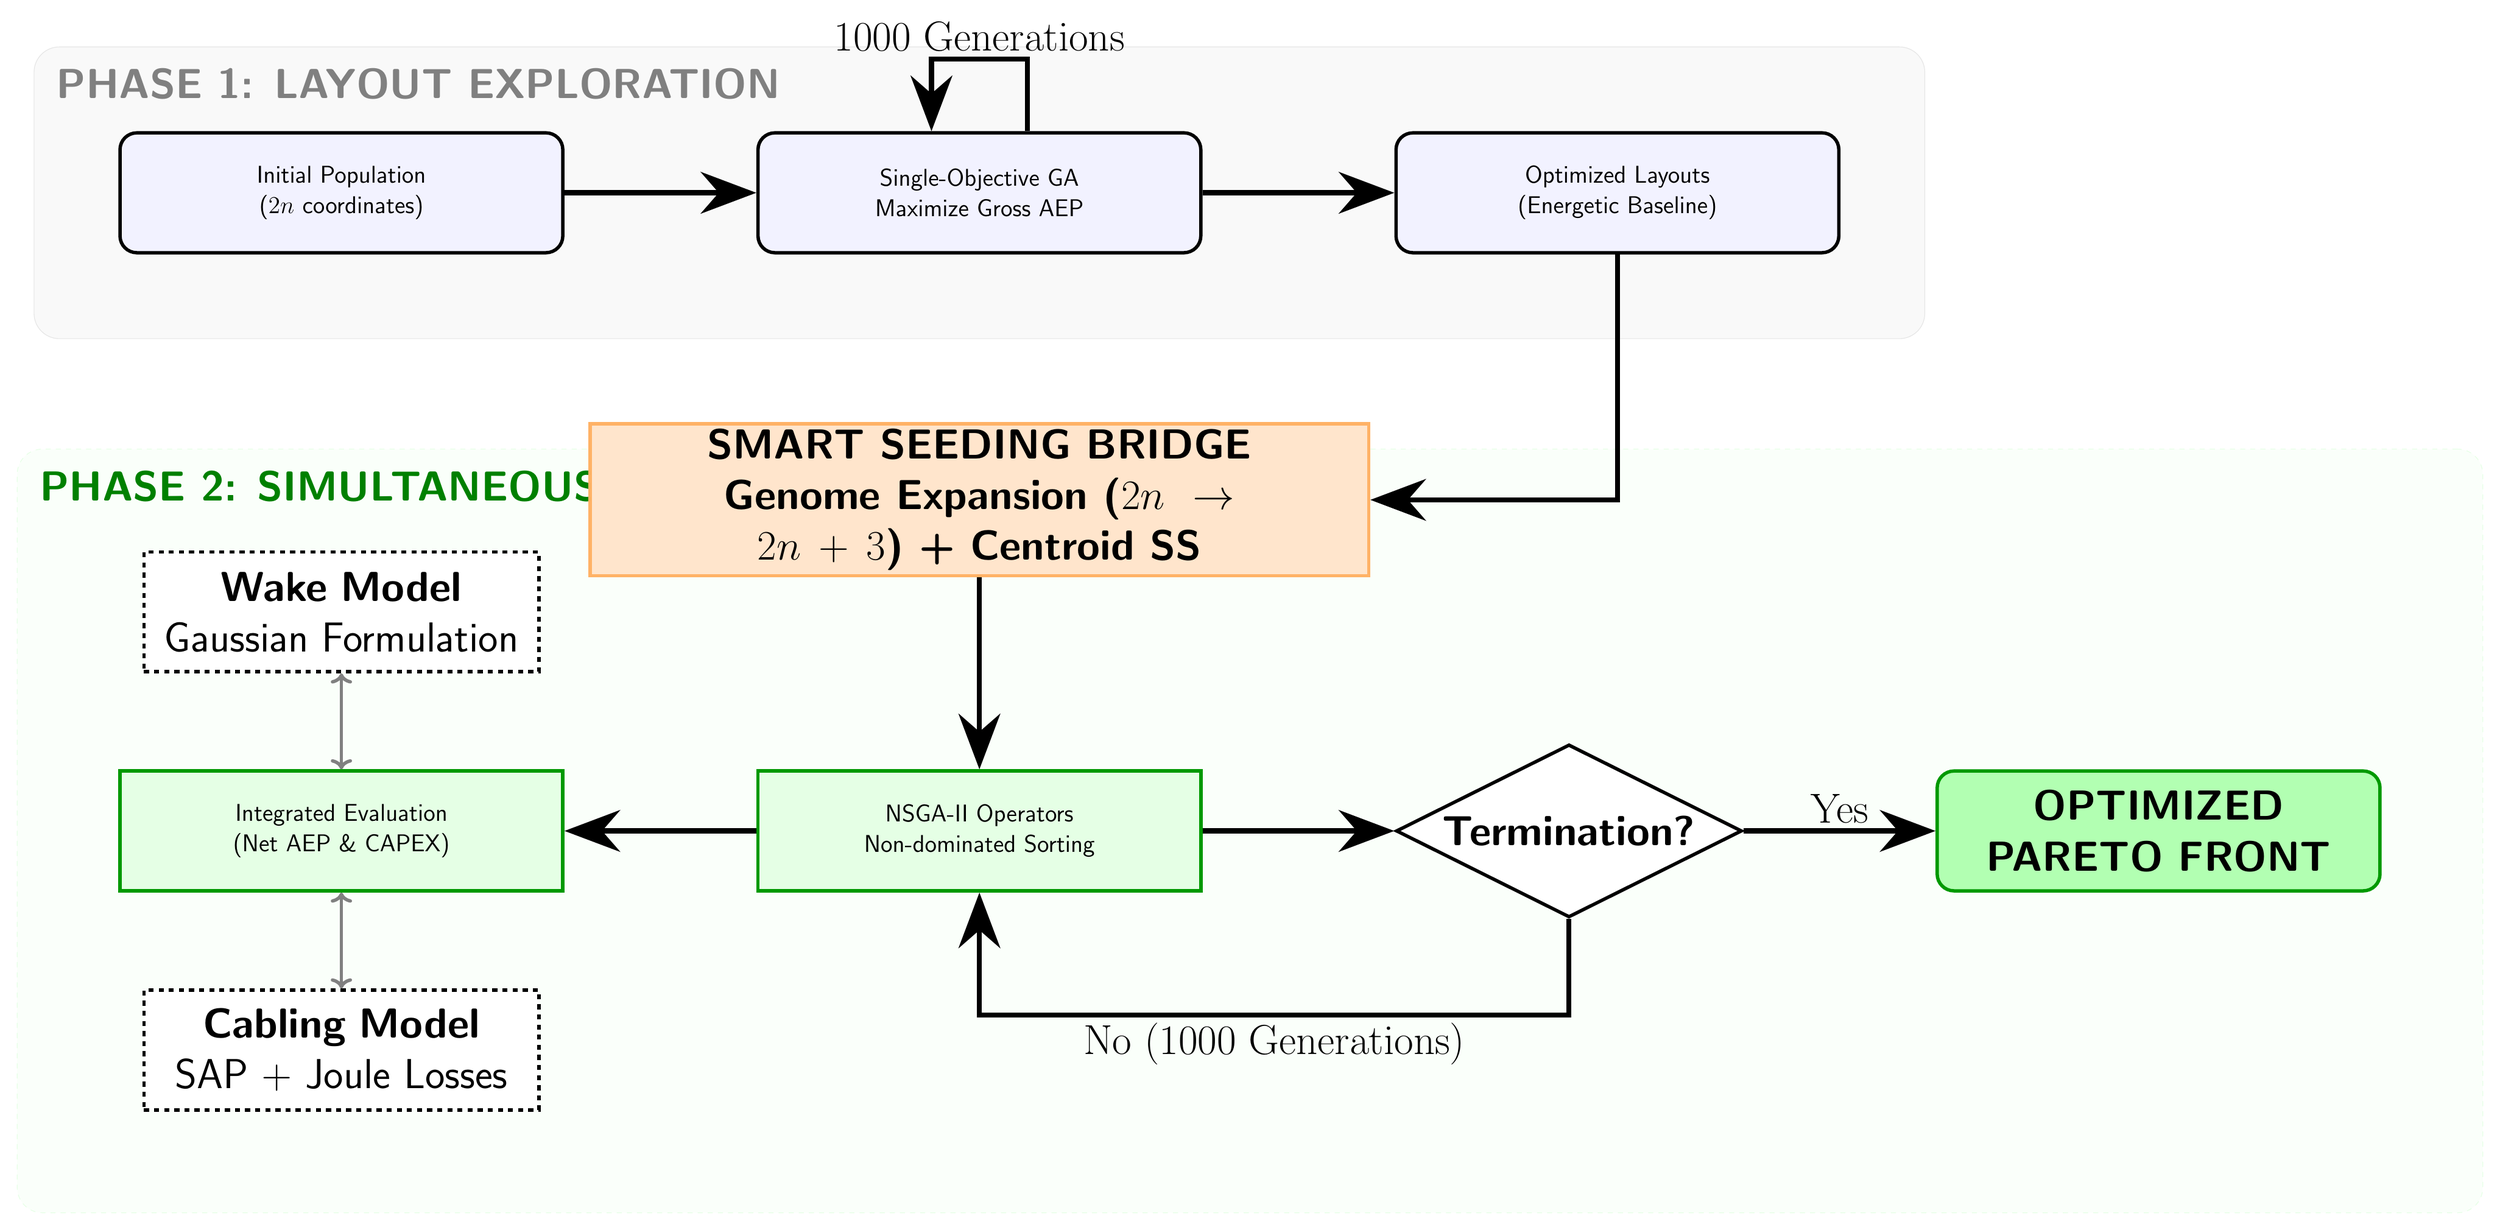
\begin{tikzpicture}[
      node distance = 2.5cm and 4cm,
      font=\sffamily\Large, % Fonte base aumentada para Huge
      base/.style = {draw, line width=2pt, text centered, minimum height=2.5cm},
      % --- Estilos de Blocos ---
      p1/.style = {base, rectangle, rounded corners=10pt, fill=blue!5, text width=9cm},
      seed/.style = {base, rectangle, fill=orange!20, text width=16cm, font=\sffamily\Huge\bfseries, draw=orange!60},
      p2/.style = {base, rectangle, fill=green!10, text width=9cm, draw=green!60!black},
      model/.style = {base, rectangle, dashed, fill=white, text width=8cm, font=\sffamily\Huge},
      decision/.style = {base, diamond, aspect=2, fill=white, inner sep=0pt, text width=6cm, font=\sffamily\Huge\bfseries},
      output/.style = {base, rectangle, rounded corners=10pt, fill=green!30, draw=green!60!black, text width=9cm, font=\sffamily\Huge\bfseries},
      arrow/.style = {line width=3pt, -{Stealth[scale=2]}}
    ]

      % --- FASE 1: LAYOUT EXPLORATION ---
      \node [p1] (init1) {Initial Population\\($2n$ coordinates)};
      \node [p1, right=of init1] (ga1) {Single-Objective GA\\Maximize Gross AEP};
      \node [p1, right=of ga1] (best1) {Optimized Layouts\\(Energetic Baseline)};

      \draw [arrow] (init1) -- (ga1);
      \draw [arrow] (ga1) -- (best1);
      % Loop da P1
      \draw [arrow] ($(ga1.north)+(1,0)$) -- ++(0,1.5) -| node[pos=0.25, anchor=south, font=\Huge] {1000 Generations} ($(ga1.north)-(1,0)$);

      % --- TRANSIÇÃO: SMART SEEDING ---
      \node [seed, below=3.5cm of ga1] (trans) {SMART SEEDING BRIDGE\\Genome Expansion ($2n \rightarrow 2n+3$) + Centroid SS};
      \draw [arrow] (best1.south) |- (trans.east);

      % --- FASE 2: CO-DESIGN ---
      \node [p2, below=4cm of trans] (ops2) {NSGA-II Operators\\Non-dominated Sorting};
      \node [p2, left=of ops2] (eval2) {Integrated Evaluation\\(Net AEP \& CAPEX)};
      
      % Modelos acoplados (Wake e Cabling)
      \node [model, above=2cm of eval2] (sim) {\textbf{Wake Model}\\Gaussian Formulation};
      \node [model, below=2cm of eval2] (cab) {\textbf{Cabling Model}\\SAP + Joule Losses};
      \draw [arrow, gray, <->, line width=2pt] (sim.south) -- (eval2.north);
      \draw [arrow, gray, <->, line width=2pt] (cab.north) -- (eval2.south);

      \node [decision, right=of ops2] (term) {Termination?};
      \node [output, right=of term] (res) {OPTIMIZED \\ PARETO FRONT};

      % Conexões P2
      \draw [arrow] (trans.south) -- (ops2.north);
      \draw [arrow] (ops2) -- (eval2);
      \draw [arrow] (ops2) -- (term);
      \draw [arrow] (term.east) -- node[anchor=south, font=\Huge] {Yes} (res.west);
      \draw [arrow] (term.south) -- ++(0,-2) -| node[pos=0.25, anchor=north, font=\Huge] {No (1000 Generations)} (ops2.south);

      % --- Containers de Fundo (Labels das Fases) ---
      \begin{scope}[on background layer]
        \node[fill=gray!5, draw=gray!20, rounded corners=15pt, inner sep=50pt, fit=(init1) (best1)] (box1) {};
        \node[fill=green!2, draw=green!10, dashed, rounded corners=15pt, inner sep=60pt, fit=(ops2) (eval2) (res) (sim) (cab)] (box2) {};
        
        \node[anchor=north west, font=\sffamily\Huge\bfseries\color{gray}, yshift=-10pt, xshift=10pt] at (box1.north west) {PHASE 1: LAYOUT EXPLORATION};
        \node[anchor=north west, font=\sffamily\Huge\bfseries\color{green!50!black}, yshift=-10pt, xshift=10pt] at (box2.north west) {PHASE 2: SIMULTANEOUS CO-DESIGN};
      \end{scope}

    \end{tikzpicture}
  }
  \caption{Proposed hierarchical evolutionary framework. Phase 1 performs an energetic search in the $2n$ spatial domain, while Phase 2 executes the multidisciplinary co-design loop using the Smart Seeding mechanism to bridge both optimization stages.}
  \label{fig:framework_diagram}
\end{figure*}

This work formulates offshore wind farm (OWF) design as a multi-objective co-design problem coupling aerodynamic performance and electrical infrastructure cost \cite{Wang2019Integrated, Jin2025Integrated}. Three evolutionary optimization strategies are compared under a unified modeling framework: a single-phase NSGA-II baseline \cite{Deb2002NSGA2}, a sequential optimization approach \cite{Moon2015Optimal, Jin2019PowerLoss}, and a two-phase hierarchical framework, originally proposed in \cite{Silva2025Layout, Silva2025b}, extended in this work to include electrical cabling.

\subsection{Problem Definition and Decision Variables}

The OWF co-design problem is represented by the decision vector
\begin{equation}
\mathbf{X} = [x_1, y_1, \dots, x_n, y_n, G_{norm}, SS_x, SS_y],
\end{equation}
where $(x_i, y_i)$ denote turbine coordinates, $(SS_x, SS_y)$ is the offshore substation position, and $G_{norm} \in [0,1]$ is a continuous grouping gene mapped to an integer number of collector strings $N_{groups} \in [N_{min}, N_{max}]$.  
This encoding enables standard continuous evolutionary operators while implicitly handling the mixed-integer nature of the design problem \cite{Haupt2004}.

\subsection{Optimization Strategies}

Three optimization paradigms are evaluated:

\textbf{Baseline (Single-Phase NSGA-II):}  
A pure NSGA-II formulation~\cite{Deb2002NSGA2} jointly optimizes Net AEP and cabling CAPEX from the initial population, evolving all decision variables simultaneously.

\textbf{Sequential Optimization:}  
A single-objective GA first optimizes turbine placement to maximize gross AEP. The resulting best layout is then fixed, and a second GA optimizes substation location and cable grouping to minimize electrical cost.

\textbf{Proposed Two-Phase Hierarchical Strategy:} 
This approach, illustrated in Fig. \ref{fig:framework_diagram}, handles the high dimensionality of the co-design problem through a structured transition between energetic and infrastructure optimization. 
Phase~1 applies a single-objective GA to maximize gross AEP over the reduced $2n$-dimensional layout space, ignoring electrical effects to promote rapid exploration.  
As depicted in the transition bridge of the framework, Phase~2 initializes its population using the best layouts from Phase~1 (Smart Seeding). Substation positions are initialized at each layout’s centroid and randomly perturbed to preserve diversity. NSGA-II then optimizes Net AEP and CAPEX over the full $2n+3$ decision vector.

\subsection{Deterministic Cabling via Strict Angular Partitioning}

To construct feasible, non-crossing electrical collection systems without geometric repair \cite{Alencar2026Flexible, Ye2023Path}, a deterministic topology synthesis mechanism termed \textit{Strict Angular Partitioning (SAP)} is adopted.  This mechanism, integrated into the multi-objective evaluation loop shown in Fig. \ref{fig:framework_diagram}, transforms the expanded decision vector into a valid collection network. For a given substation position, turbines are sorted by polar angle, partitioned into contiguous angular sectors according to $N_{groups}$, and connected radially from the outermost turbines toward the substation.  
This guarantees planar cable layouts and enables efficient evaluation within the evolutionary loop.

\subsection{Objective Functions}

The three optimization strategies employ different objective function configurations across their respective phases. The fundamental objectives considered are:

\textbf{Objective 1 — Maximize Net AEP:}
\begin{equation}
f_1(\mathbf{X}) = \text{AEP}_{gross} - \mathcal{L}_{joule},
\end{equation}
where gross AEP is computed using a Gaussian wake model \cite{Bastankhah2014Gaussian, Bastankhah2016Gaussian} and $\mathcal{L}_{joule}$ represents electrical Joule losses in the collection system. This objective requires simultaneous evaluation of turbine layout and electrical infrastructure, as cable routing determines $\mathcal{L}_{joule}$.



\textbf{Objective 2 — Minimize Cabling CAPEX:}
\begin{equation}
f_2(\mathbf{X}) = \sum_{c=1}^{N_{cables}} L_c \cdot C(CSA_{uniform}),
\end{equation}
where $L_c$ denotes cable lengths and $C(CSA_{uniform})$ is the cost of a uniformly selected commercial cable cross-section \cite{Nakhai2023Electrical}.

\textbf{Baseline (Single-Phase NSGA-II):} Both objectives $f_1$ (Net AEP) and $f_2$ (Cabling CAPEX) are optimized simultaneously from the initial population using NSGA-II \cite{Deb2002NSGA2}, evolving all decision variables ($2n+3$) concurrently throughout the entire optimization process. Since cable routing is evaluated at each generation, $\mathcal{L}_{joule}$ is explicitly accounted for in $f_1$.

\textbf{Sequential Optimization:} Phase~1 applies a single-objective GA to maximize gross AEP over the $2n$-dimensional layout space, ignoring electrical infrastructure entirely. The objective function is simply $\text{AEP}_{gross}$ (without $\mathcal{L}_{joule}$), as cable routing is not evaluated at this stage. The resulting best layout is then fixed, and Phase~2 employs a second single-objective GA to minimize $f_2$ (cabling CAPEX) by optimizing substation location and cable grouping variables only, with turbine positions held constant.

\textbf{Proposed Two-Phase Hierarchical Strategy:} Phase~1 applies a single-objective GA to maximize gross AEP over the reduced $2n$-dimensional layout space, using the same objective as Sequential Phase~1 (gross AEP only, without electrical losses). Phase~2 initializes its population using the best layouts from Phase~1 (Smart Seeding) and employs NSGA-II \cite{Deb2002NSGA2} to simultaneously optimize both $f_1$ (Net AEP, including $\mathcal{L}_{joule}$) and $f_2$ (Cabling CAPEX) over the full $2n+3$ decision vector, enabling explicit exploration of energy--cost trade-offs while allowing turbine repositioning to account for electrical infrastructure effects.

\subsection{Case Study Configuration}

All strategies are evaluated on a reference offshore wind farm design problem derived from the IEA Task~37 benchmark \cite{Baker2019Best}. A fixed wind regime with constant wind speed of 9.8\,m/s (rated speed) and a standard 3.35\,MW reference turbine are adopted. Experiments are conducted for three problem scales (16, 36, and 64 turbines) within a fixed circular site of 5000\,m radius, with a minimum inter-turbine distance constraint of 2 rotor diameters (260\,m). This configuration enables controlled comparison of solution quality, convergence behavior, and computational cost across increasing problem dimensionality.


\subsection{Experimental Design and Evaluation Protocol}
\label{sec:experimental_design}

The goal of the experimental design is not only to assess solution quality, but to analyze how different evolutionary optimization paradigms affect convergence behavior, diversity preservation, and trade-off exploration in a coupled aerodynamic--electrical design problem.

All optimization strategies are evaluated under identical computational budgets, population sizes, and initial conditions to ensure a fair comparison. Each strategy uses a population size of 300 individuals and equivalent computational budgets: Baseline executes 2000 generations, while Sequential and Proposed each execute 1000 generations in Phase~1 followed by 1000 generations in Phase~2, totaling 2000 generations per strategy. To ensure fair comparison, all methods share the same global initial population for each independent run. Twenty independent runs are performed for each strategy, with each run using a unique random seed that is shared across all methods, following best practices in evolutionary computation \cite{Deb2002NSGA2, Haupt2004}.

Performance is assessed using both objective-space and algorithmic metrics. In addition to Net AEP and cabling CAPEX, the following indicators are considered: (i) the number of non-dominated solutions, (ii) Pareto front spread, and (iii) hypervolume (HV). Hypervolume is adopted as the primary performance indicator due to its ability to simultaneously capture convergence and diversity, making it particularly suitable for engineering design trade-offs \cite{Deb2002NSGA2}.

Computational efficiency is also reported, as scalability remains a key concern in real-world offshore wind farm design, where the dimensionality of the search space grows linearly with the number of turbines. This is especially relevant when comparing single-phase and decomposed optimization strategies operating in spaces of dimension $2n$ versus $2n+3$.

\section{Results and Discussion}
\label{sec:results}

This section presents a comprehensive comparison of three evolutionary optimization strategies, Baseline NSGA-II, Sequential optimization, and the Proposed two-phase hierarchical framework, evaluated across increasing problem scales (16, 36, and 64 turbines). The analysis combines quantitative multi-objective performance indicators with qualitative inspection of Pareto-optimal layouts to assess how problem decomposition, search dimensionality, and evolutionary strategy influence scalability, convergence behavior, robustness, and trade-off resolution. Similar comparative and scale-aware analyses have been identified as essential for assessing practical relevance in recent WFLO and integrated OWF design studies \cite{Jiang2025Review, Tao2025TwoStage}.

\subsection{Quantitative Performance Across Problem Scales}

Table~\ref{tab:quantitative_summary} summarizes the main performance indicators obtained for the three turbine densities. Across all scenarios, the Sequential strategy consistently converges to a single solution. This outcome is a direct consequence of its single-objective decomposition and fixed-layout assumption, which precludes the emergence of Pareto fronts and prevents explicit exploration of energy--cost trade-offs. Similar limitations of sequential or partially fixed approaches have been reported in earlier WFLO--WFCRP studies \cite{Fischetti2015MILP, Moon2015Optimal}.

Both the Baseline NSGA-II and the Proposed framework generate non-dominated solution sets; however, important differences emerge. For the 16-turbine scenario, the Baseline strategy achieves Net AEP ranging from 389.31 to 418.93 GWh, while the Proposed framework achieves a higher and narrower range from 453.43 to 461.32 GWh, indicating superior exploration of high-AEP regions. The Proposed framework consistently achieves higher HV values (8.99 vs 8.52 $\times 10^{12}$), reflecting improved coverage of infrastructure-driven trade-offs and greater diversity in the Pareto front.

As the problem size increases to 36 turbines, the Baseline NSGA-II exhibits a marked degradation in Pareto front quality, with reduced hypervolume (16.34 vs 17.30 $\times 10^{12}$ for Proposed) and increased variability in Pareto front cardinality. The Baseline strategy achieves Net AEP ranging from 822.61 to 853.66 GWh, while the Proposed framework achieves a higher range from 932.42 to 951.27 GWh, maintaining superior exploration of high-AEP regions. The Proposed framework's HV advantage increases from 5.5\% at 16 turbines to 5.9\% at 36 turbines, demonstrating improved scalability. This behavior is consistent with well-known scalability limitations of fully coupled evolutionary searches in high-dimensional design spaces \cite{Haupt2004, Nocedal2006}. In contrast, the Proposed two-phase strategy maintains stable Pareto diversity and superior objective-space coverage, demonstrating increased robustness to dimensionality growth.

For the 64-turbine scenario, the scalability advantages of the Proposed framework become even more pronounced. The Baseline strategy achieves Net AEP ranging from 1292.08 to 1351.85 GWh, while the Proposed framework achieves a higher range from 1400.44 to 1489.04 GWh, representing an 8.9\% improvement in mean Net AEP. However, at this scale, both strategies exhibit issues with hypervolume calculation reliability that appear to be seed-dependent rather than method-specific. The Baseline strategy shows hypervolume values near zero for all runs, while the Proposed framework maintains valid hypervolume values (22.50 $\times 10^{12}$) for approximately half of the runs, with the remaining runs also exhibiting calculation issues. This seed-dependent behavior suggests that certain initializations may lead to convergence difficulties in high-dimensional spaces, affecting both strategies to varying degrees. Notably, the Proposed framework produces fewer Pareto solutions at this scale (mean: 2 vs 297 at 16 turbines) for runs with valid hypervolume, which may indicate aggressive convergence to high-performance regions or premature convergence. Despite this reduction in solution diversity, the high hypervolume values for valid runs suggest that the solutions found are of superior quality.

Computational efficiency analysis, shown in Figure~\ref{fig:execution_time}, reveals that the Proposed framework achieves substantial execution time reductions compared to Baseline: 31.6\% at 16 turbines (6.9 vs 10.1 minutes), 41.2\% at 36 turbines (49.2 vs 83.7 minutes), and 45.2\% at 64 turbines (90.5 vs 165.1 minutes). The Baseline strategy's execution time increases by 16.36$\times$ from 16 to 64 turbines, while the Proposed strategy shows better scalability with a 13.11$\times$ increase, confirming the computational efficiency advantages of hierarchical decomposition at larger scales. The Sequential strategy is fastest but converges to a single solution per run, precluding trade-off exploration.

\begin{table}[htbp]
\caption{Objective-space performance comparison across optimization strategies (mean $\pm$ std over independent runs: 20 for 16 turbines; 15 Baseline, 20 Sequential, 15 Proposed for 36 turbines; 10 Baseline, 20 Sequential, 16 Proposed for 64 turbines). Pareto front size, hypervolume, and execution time are shown in Figures~\ref{fig:pareto_comparison}, \ref{fig:hv_all}, and \ref{fig:execution_time}, respectively.}   
\label{tab:quantitative_summary}
\centering
\begin{tabular}{c l c c}
\toprule
\textbf{Turb.} & \textbf{Method} & \textbf{Net AEP} & \textbf{CAPEX} \\
&  & [GWh] & [kUSD] \\
\midrule
\multirow{3}{*}{16}
& Baseline   & $404.34 \pm 8.44$ & $190 \pm 22$ \\
& Sequential & $462.99 \pm 0.43$ & $731 \pm 108$ \\
& Proposed   & $457.89 \pm 2.39$ & $657 \pm 91$ \\
\midrule
\multirow{3}{*}{36}
& Baseline   & $835.10 \pm 7.30$ & $875 \pm 93$ \\
& Sequential & $944.62 \pm 3.16$ & $1838 \pm 327$ \\
& Proposed   & $941.95 \pm 5.72$ & $2013 \pm 263$ \\
\midrule
\multirow{3}{*}{64}
& Baseline   & $1329.29 \pm 17.91$ & $2416 \pm 37$ \\
& Sequential & $1503.81 \pm 12.27$ & $3325 \pm 200$ \\ 
& Proposed   & $1444.17 \pm 28.69$ & $3281 \pm 286$ \\ 
\bottomrule
\end{tabular}
\end{table}

\begin{figure}[htbp]
\centering
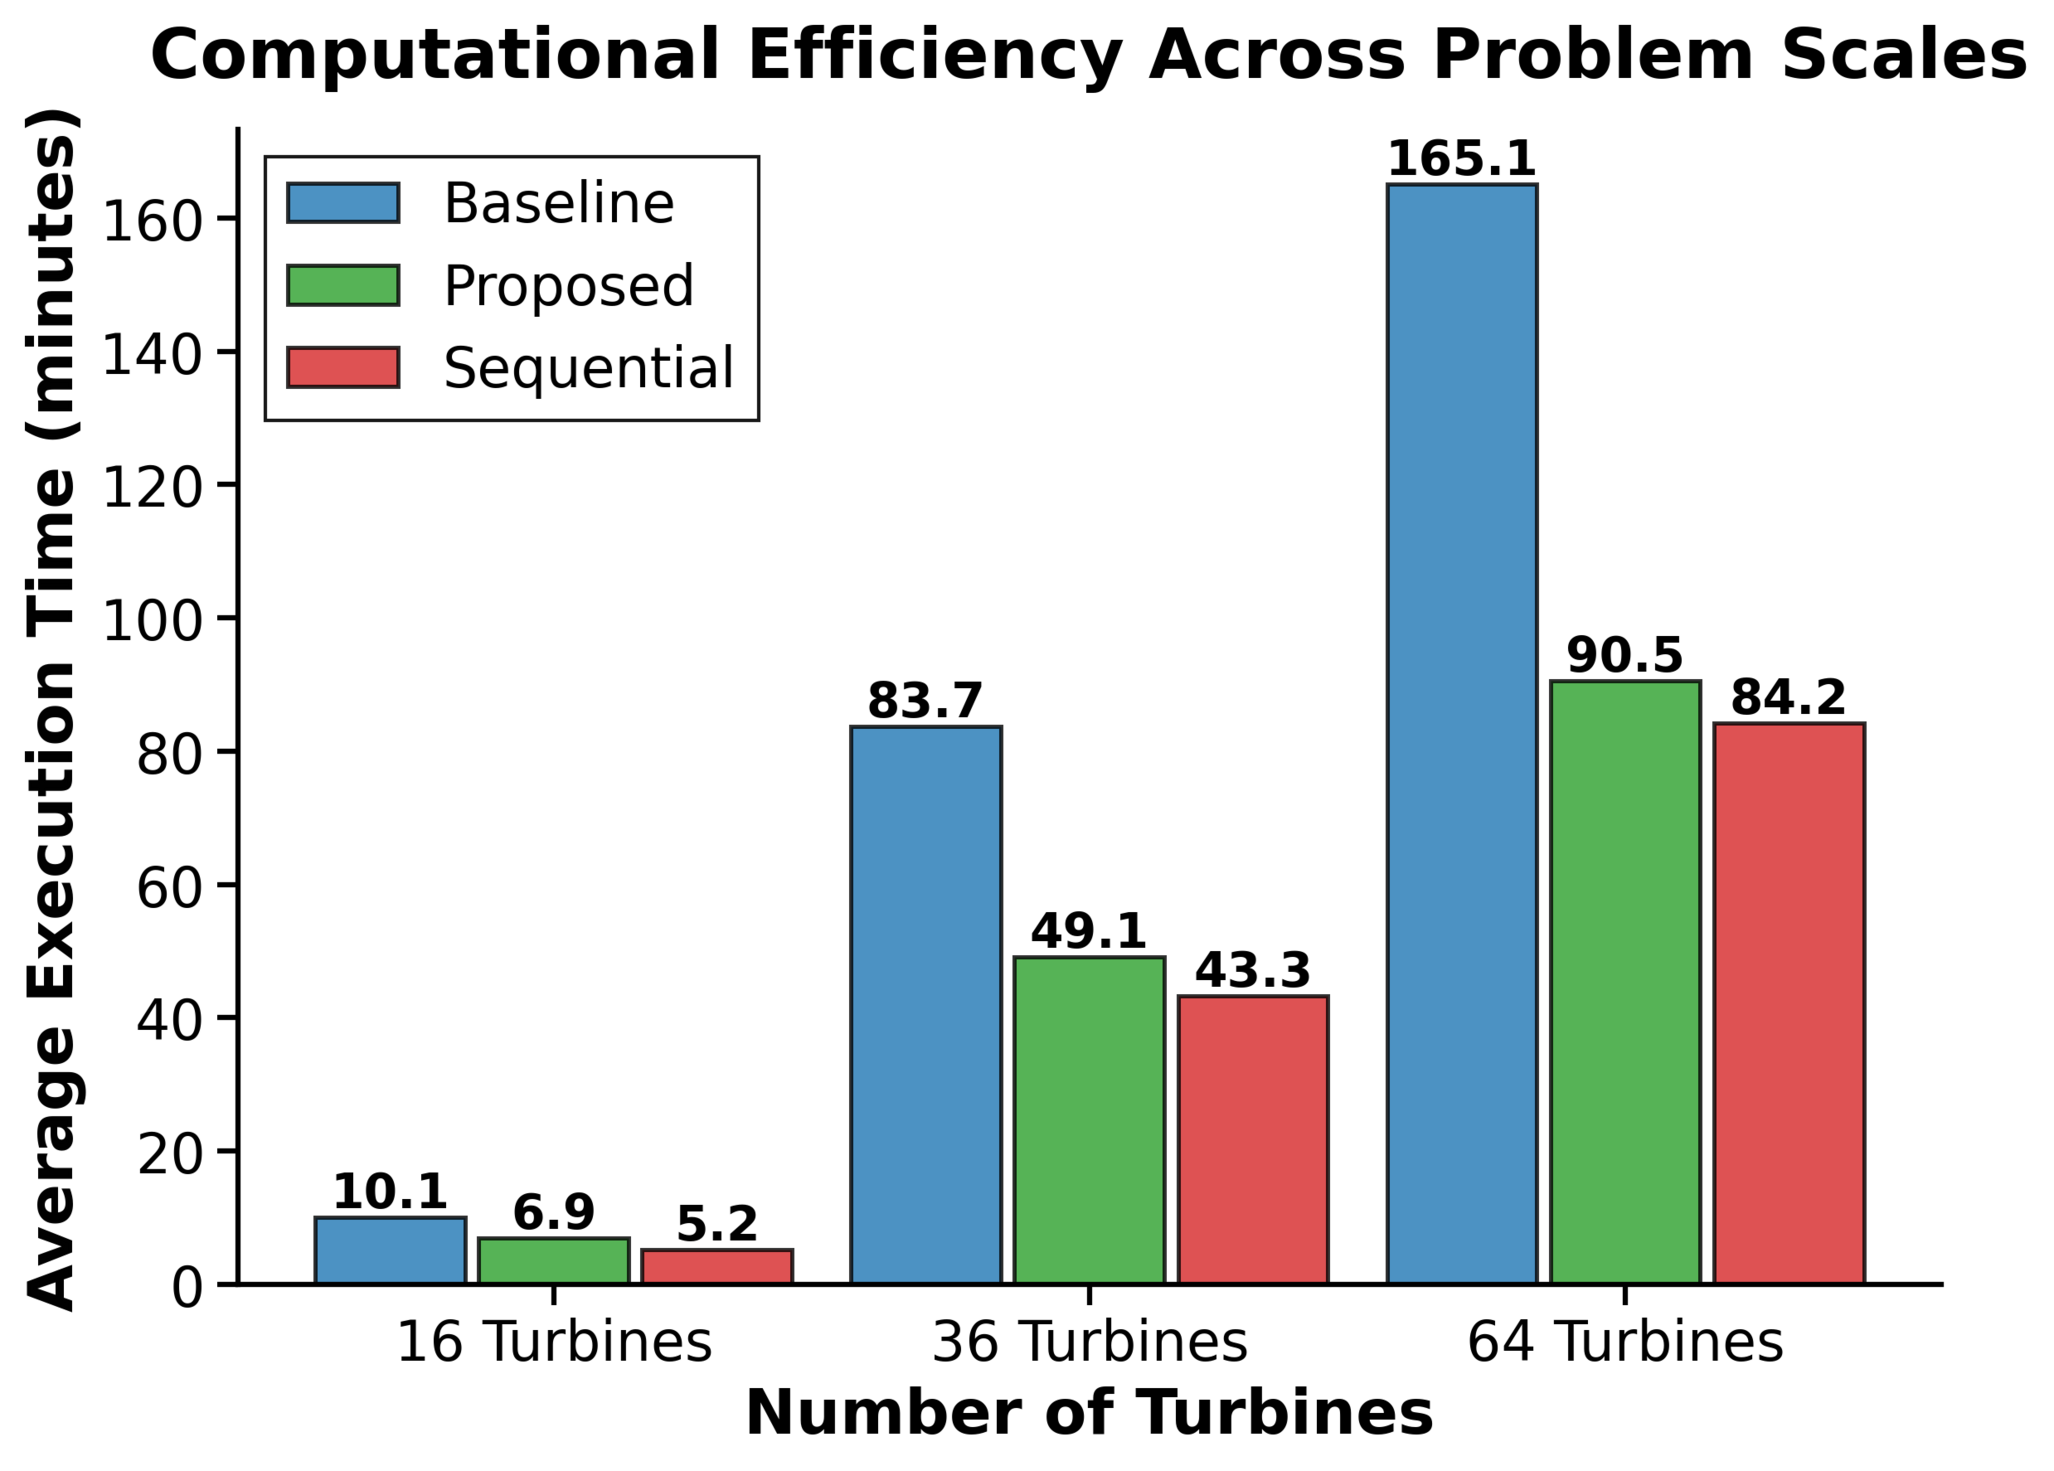
\includegraphics[width=\columnwidth]{img/execution_time_comparison.png}
\caption{Average execution time per run across optimization strategies for increasing problem scales. The Proposed framework achieves substantial reductions compared to Baseline: 31.6\% at 16 turbines (6.9 vs 10.1 minutes), 41.2\% at 36 turbines (49.2 vs 83.7 minutes), and 45.2\% at 64 turbines (90.5 vs 165.1 minutes), demonstrating superior scalability (13.11$\times$ vs 16.36$\times$ increase from 16 to 64 turbines).}
\label{fig:execution_time}
\end{figure}


\subsection{Pareto Front Structure and Trade-off Analysis}

Figure~\ref{fig:pareto_comparison} compares the Pareto fronts obtained by the three strategies across increasing problem scales. The Sequential strategy converges to a single solution per run, confirming its inability to expose trade-offs within each optimization run. In the aggregated plot, multiple Sequential points appear (one per independent run), but these represent different converged solutions rather than a Pareto front from a single run. The Baseline and Proposed strategies both generate Pareto fronts within each run; however, important differences emerge in their objective-space coverage.

For the 16-turbine scenario, as shown in Fig.~\ref{fig:pareto_16}, the Proposed framework exhibits broader coverage of the objective space, with solutions spanning a more diverse set of energy--cost trade-offs. The Baseline strategy, while achieving lower minimum cabling costs, shows more limited coverage of the Pareto-optimal region, particularly in high-energy production regimes. 

For the 36-turbine scenario, as shown in Fig.~\ref{fig:pareto_36}, the performance gap between strategies widens. The Proposed framework maintains broader coverage of high-AEP regions, while the Baseline strategy shows increased clustering of solutions and reduced coverage of low-cost regions.

For the 64-turbine scenario, as shown in Fig.~\ref{fig:pareto_64}, the Proposed framework continues to achieve superior Net AEP ranges. However, both strategies exhibit reduced Pareto front diversity at this scale, with the Proposed framework producing fewer solutions (mean: 2 vs 297 at 16 turbines), which may reflect convergence to high-performance regions or seed-dependent calculation issues. The Sequential strategy achieves the highest Net AEP but converges to a single solution per run, precluding trade-off exploration.

\begin{figure*}[htbp]
\centering
\begin{subfigure}[b]{0.33\textwidth}
    \centering
    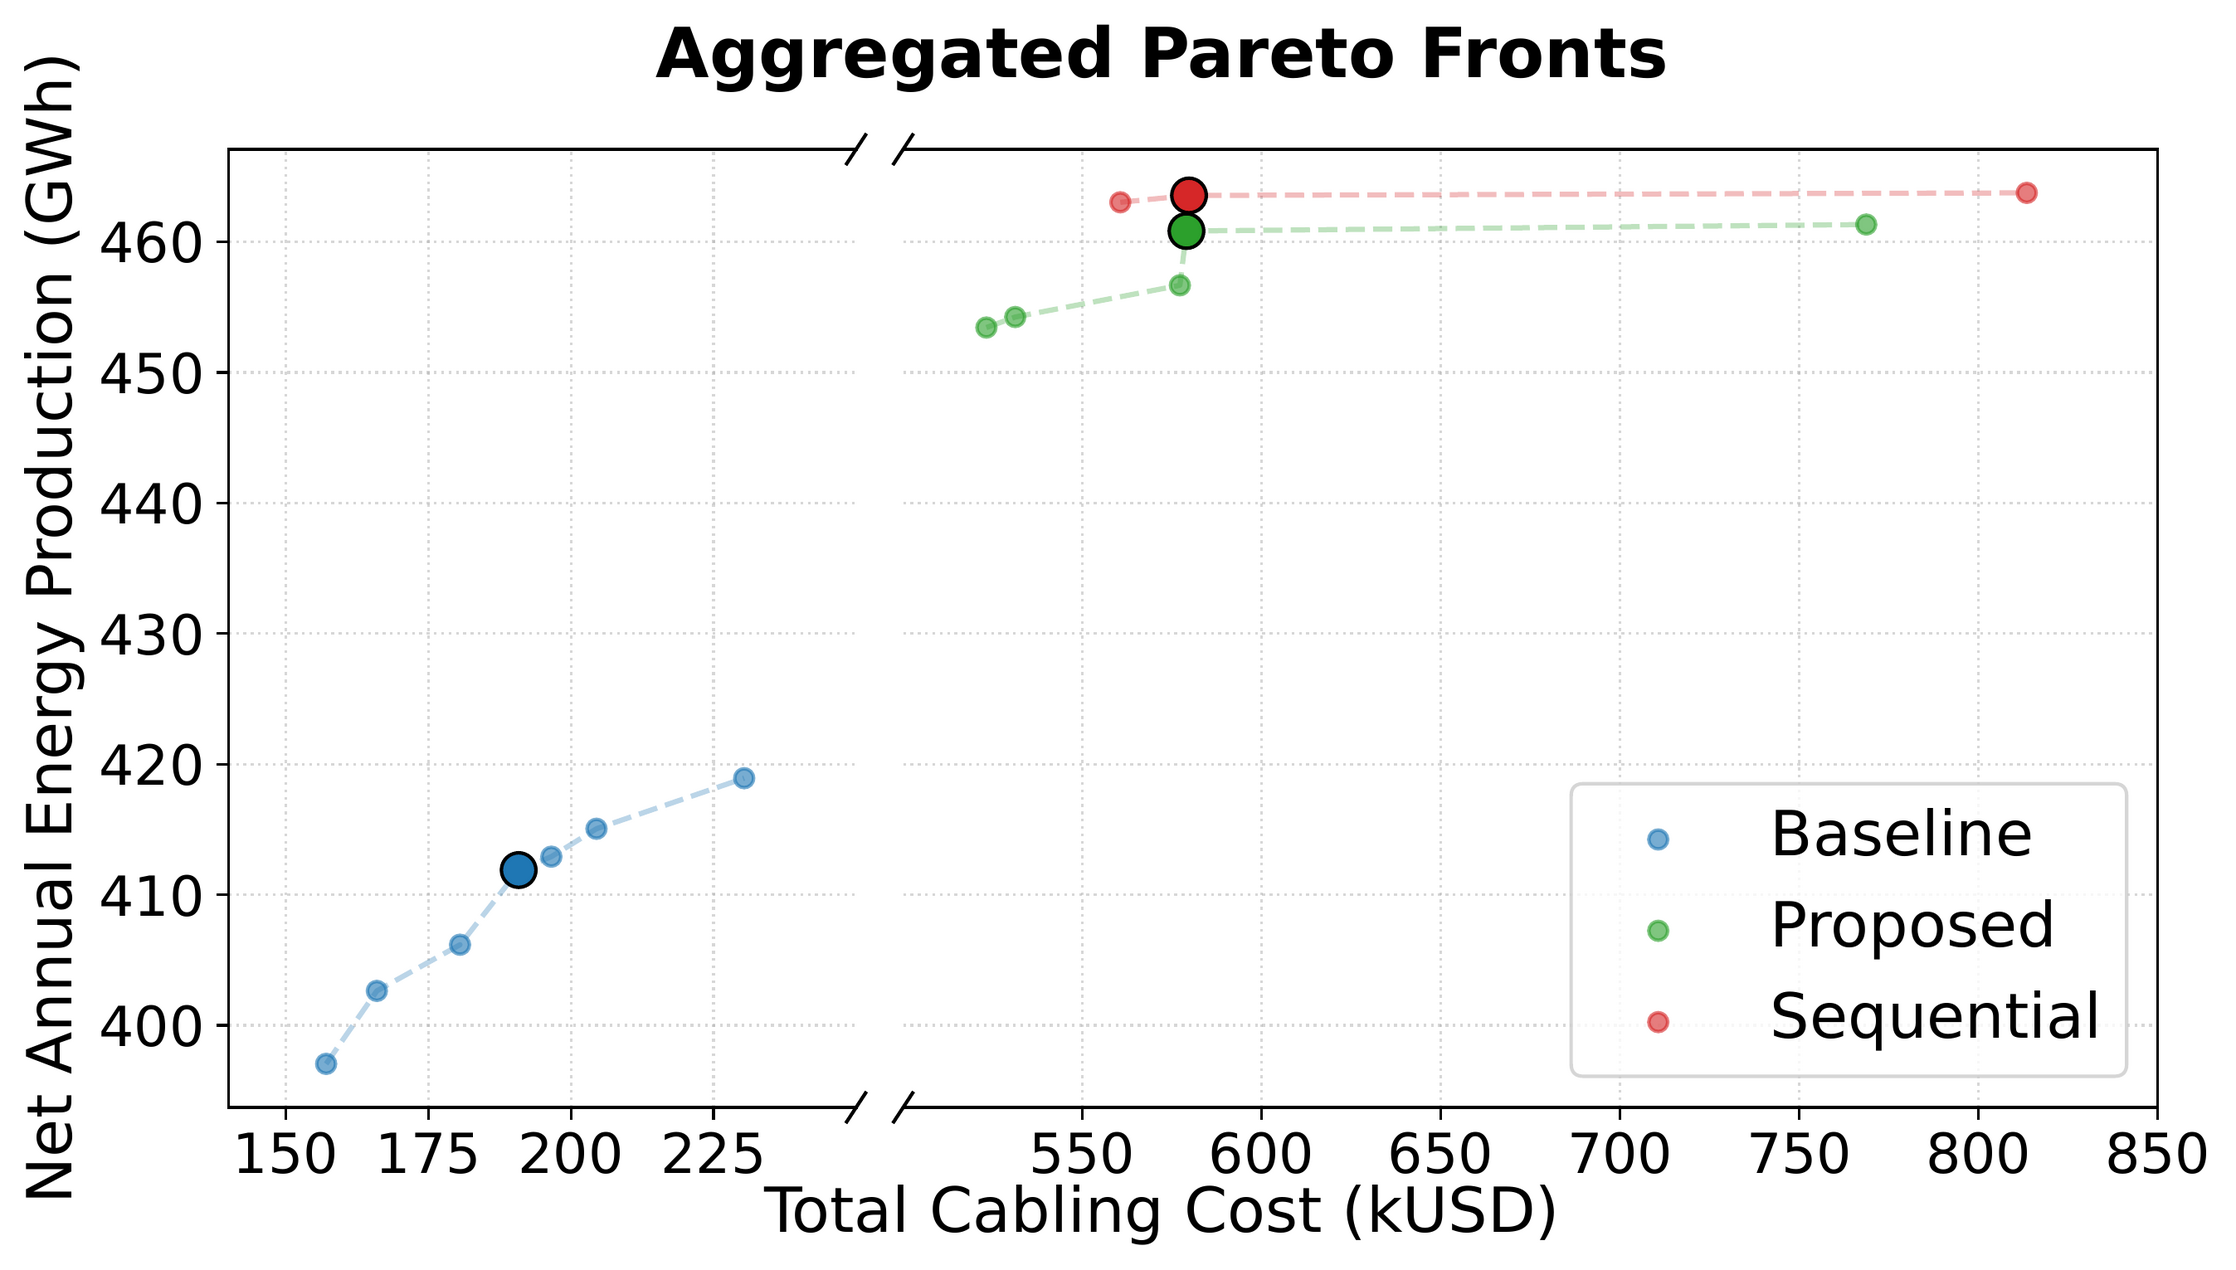
\includegraphics[width=\linewidth]{img/pareto_compacto_16.png}
    \caption{16 turbines}
    \label{fig:pareto_16}
\end{subfigure}
\hfill
\begin{subfigure}[b]{0.33\textwidth}
    \centering
    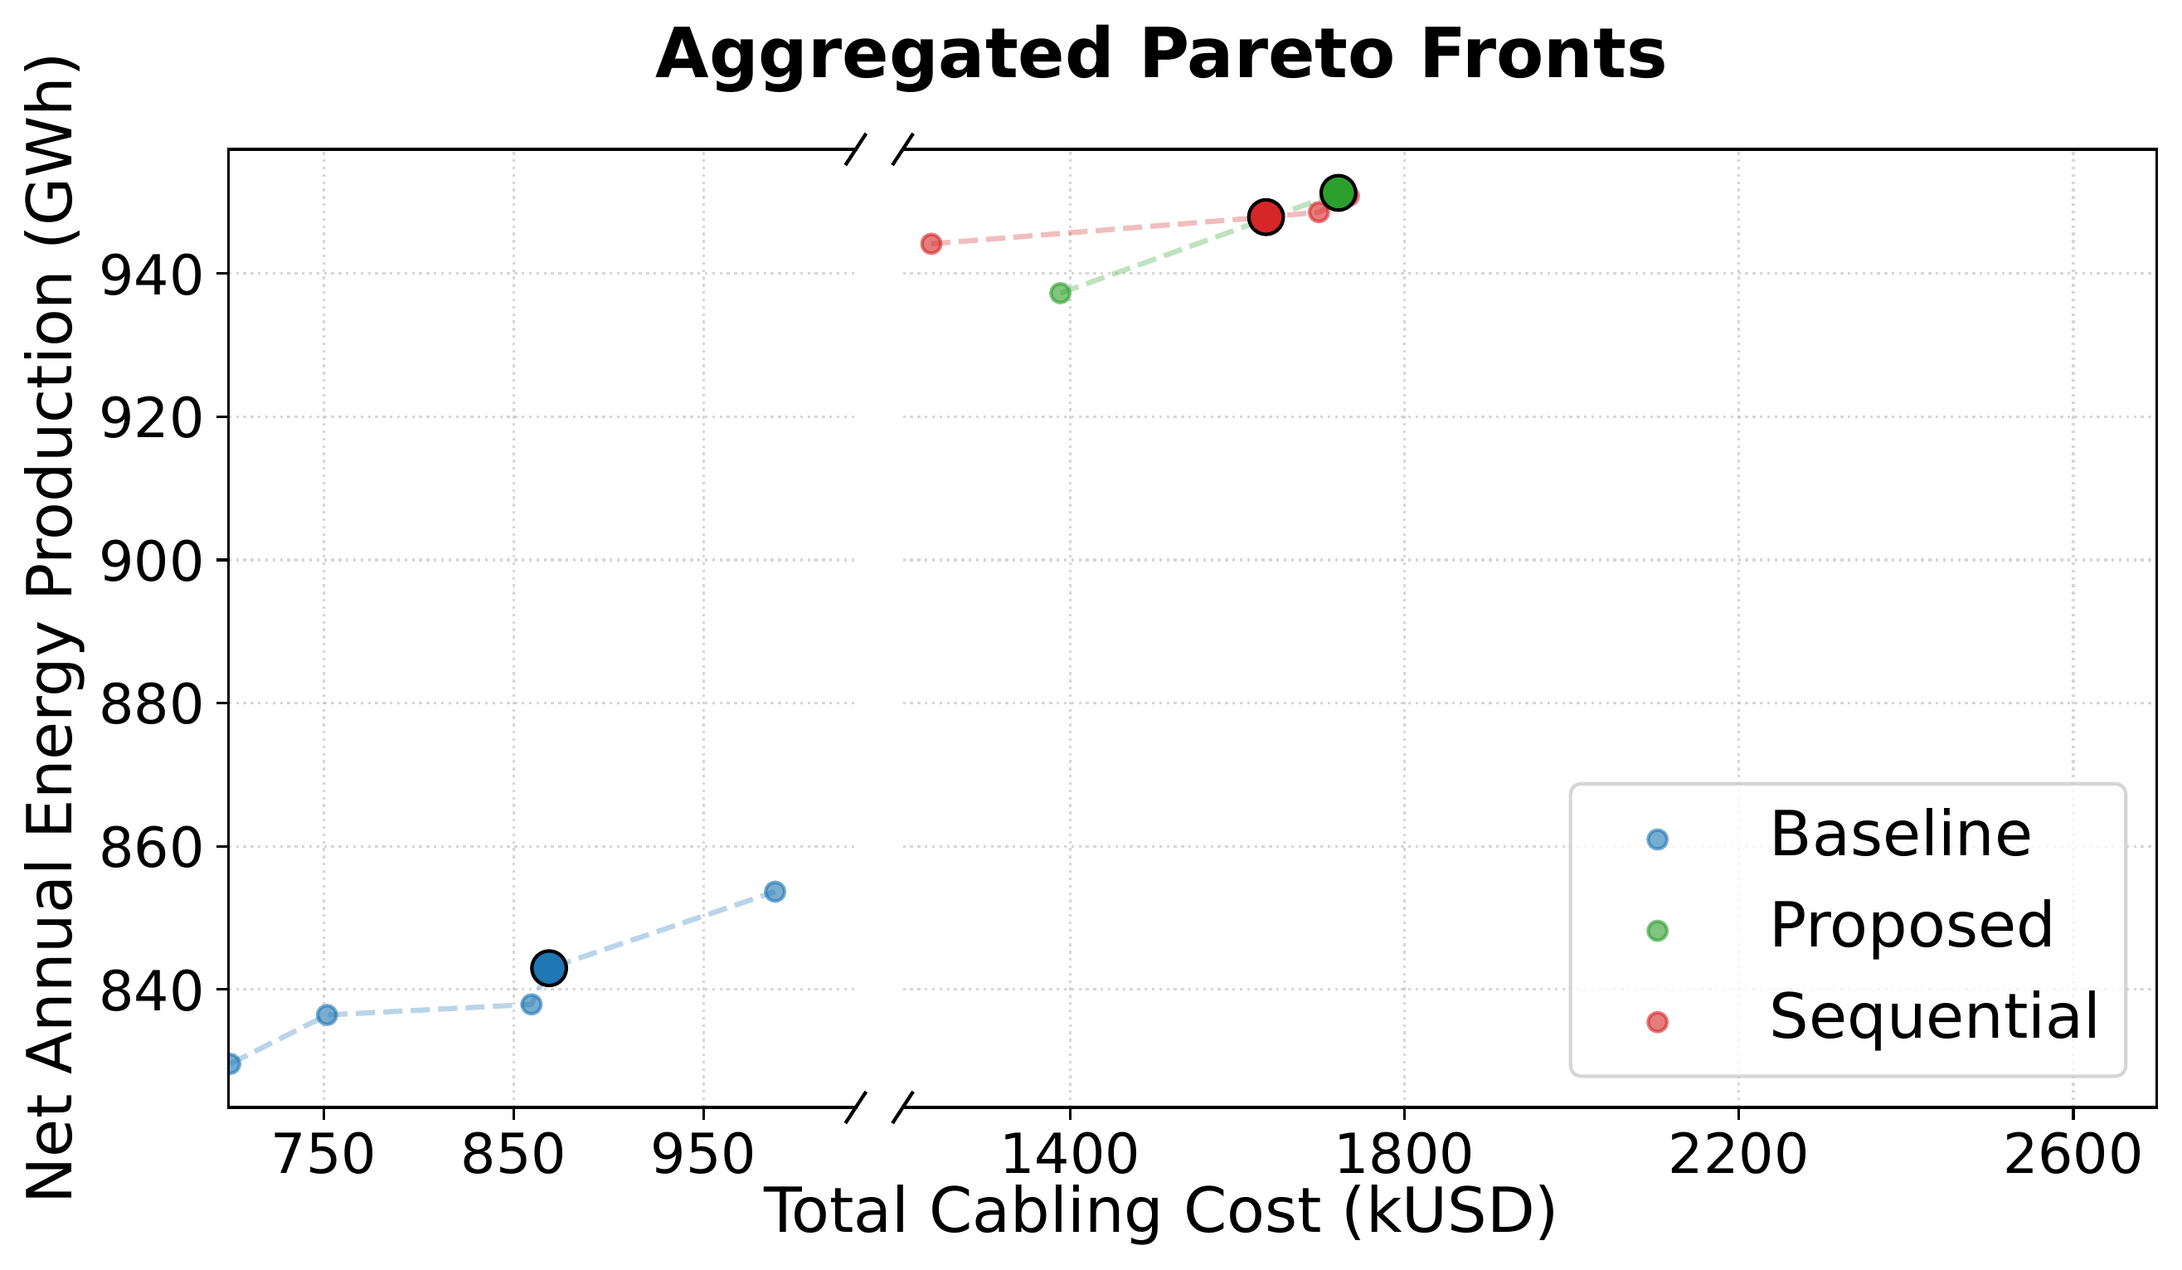
\includegraphics[width=\linewidth]{img/pareto_compacto_36.png}
    \caption{36 turbines}
    \label{fig:pareto_36}
\end{subfigure}
\hfill
\begin{subfigure}[b]{0.33\textwidth}
    \centering
    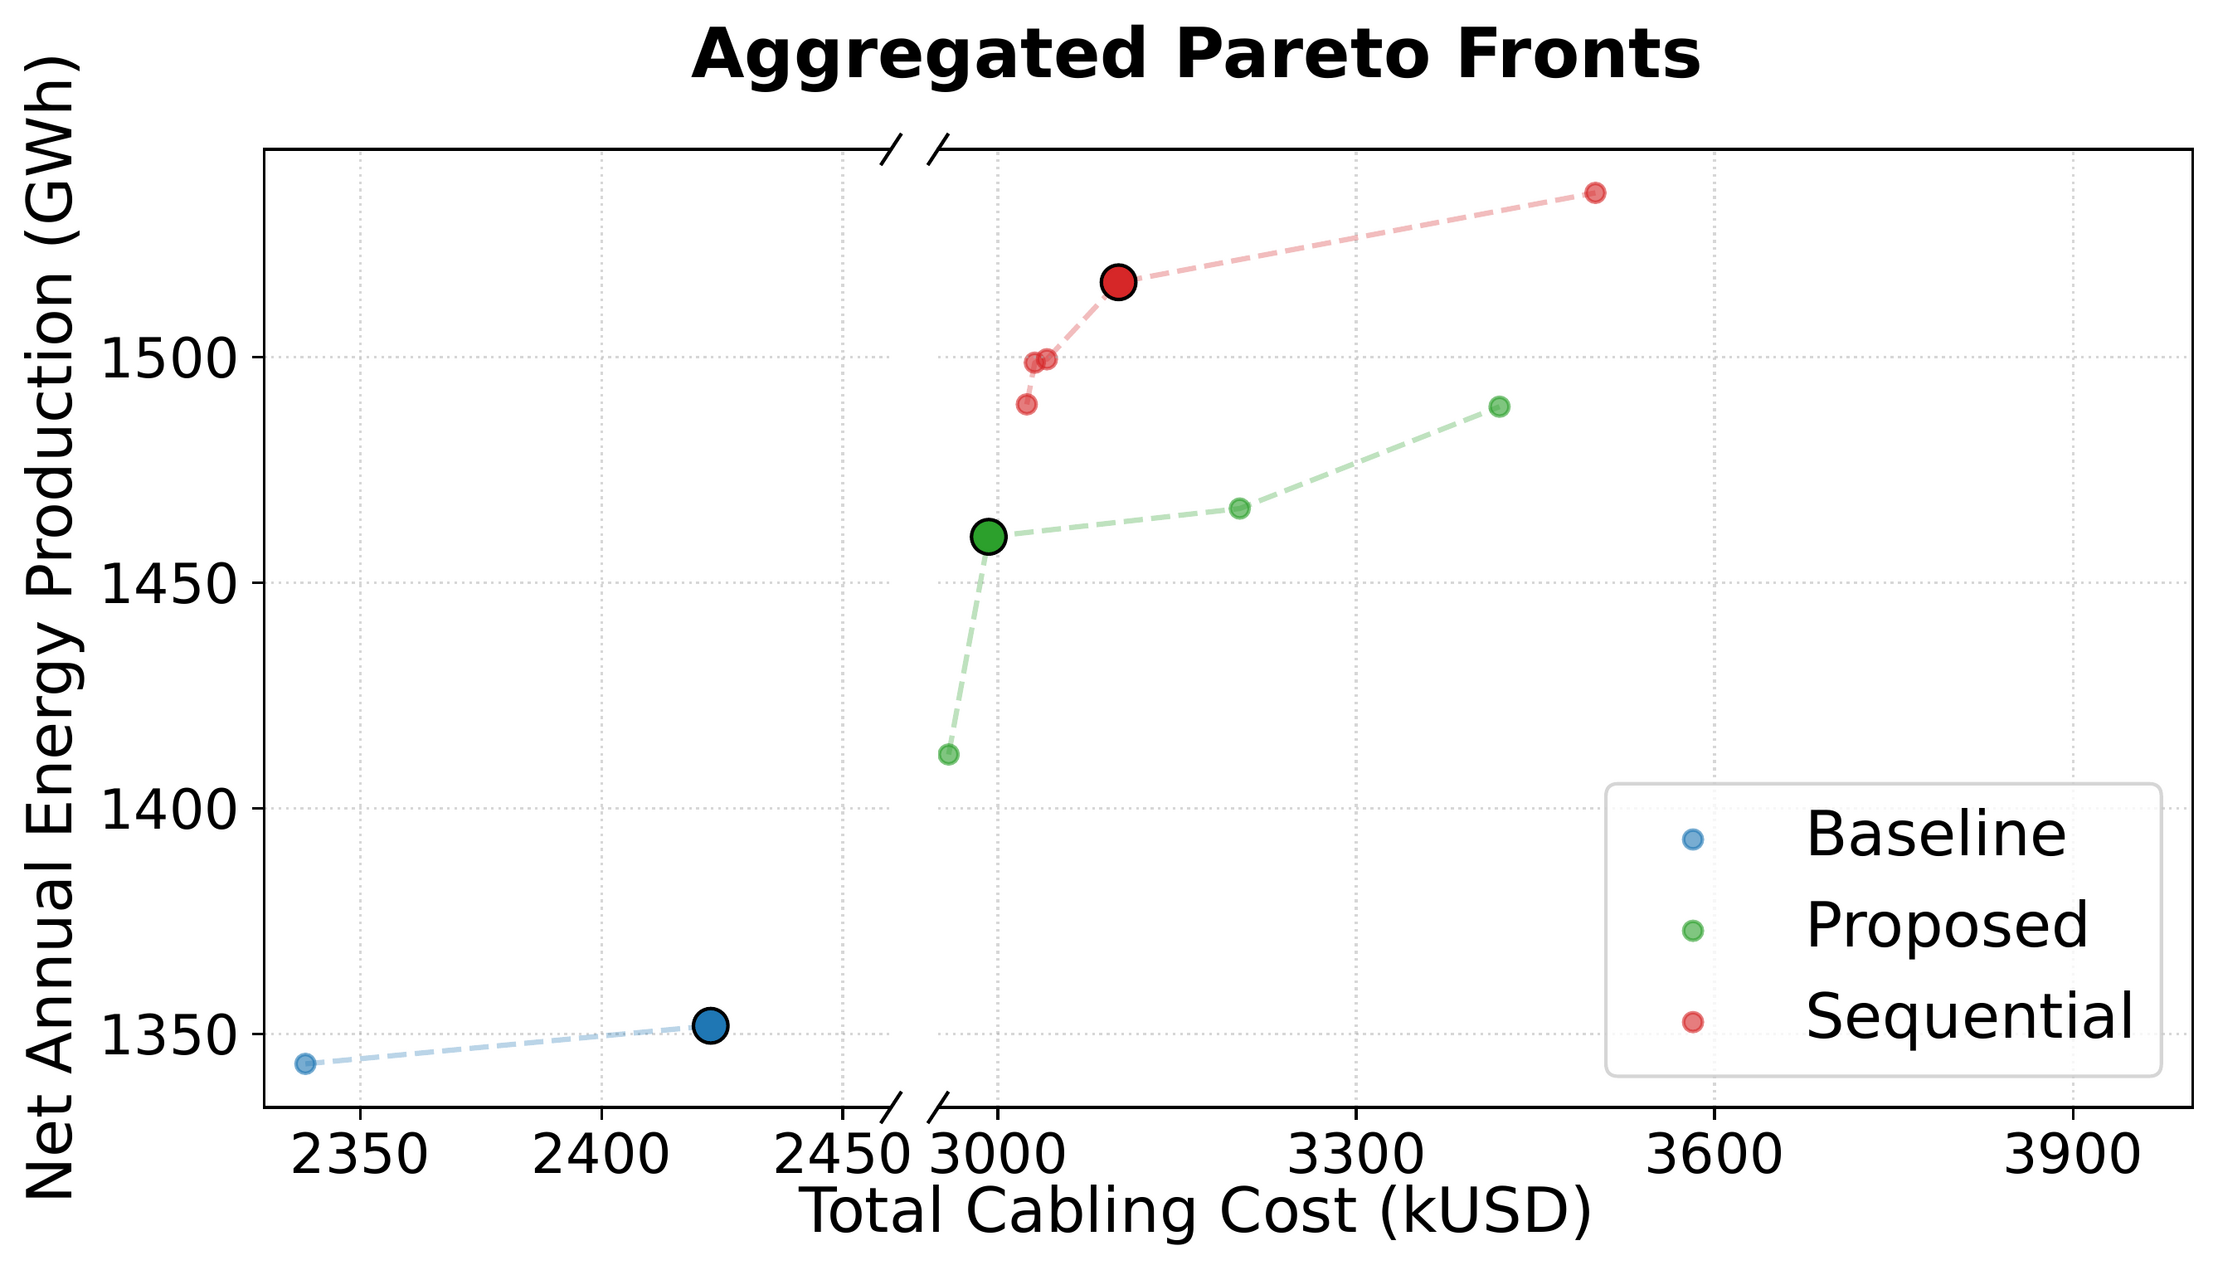
\includegraphics[width=\linewidth]{img/pareto_compacto_64.png}
    \caption{64 turbines}
    \label{fig:pareto_64}
\end{subfigure}

\caption{Pareto front comparison between Baseline NSGA-II, Sequential optimization, and the Proposed framework for increasing problem scales. The Sequential strategy converges to a single solution per run (multiple points in the aggregated plot represent different runs, not a Pareto front). The Proposed framework exhibits broader objective-space coverage at all scales, enabling exploration of diverse energy--cost trade-offs.}
\label{fig:pareto_comparison}
\end{figure*}

These results confirm that hierarchical problem decomposition enhances the algorithm's ability to resolve conflicting aerodynamic and electrical objectives, a property that becomes increasingly important as the number of decision variables grows.

\subsection{Convergence Behavior and Hypervolume Evolution}

\begin{figure*}[htbp]
     \centering
     % Subfigura 1: 16 Turbinas
     \begin{subfigure}[b]{0.32\textwidth}
         \centering
         \includegraphics[width=\linewidth]{img/hv_16_3.png}
         \caption{16 turbines}
         \label{fig:hv_16}
     \end{subfigure}
     \hfill
     % Subfigura 2: 36 Turbinas
     \begin{subfigure}[b]{0.32\textwidth}
         \centering
         \includegraphics[width=\linewidth]{img/hv_36_3.png}
         \caption{36 turbines}
         \label{fig:hv_36}
     \end{subfigure}
     \hfill
     % Subfigura 3: 64 Turbinas
     \begin{subfigure}[b]{0.32\textwidth}
         \centering
         \includegraphics[width=\linewidth]{img/hv_64_3.png}
         \caption{64 turbines}
         \label{fig:hv_64}
     \end{subfigure}
     
    \caption{Hypervolume evolution across different farm scales. The Proposed strategy consistently achieves higher hypervolume values than Baseline, with the performance advantage becoming more pronounced at larger scales. At 64 turbines, both strategies exhibit seed-dependent calculation issues, likely due to geometric constraints when routing 64 turbines with few cable groups (see Table~\ref{tab:qualitative_characteristics}) without cable crossings.}

     \label{fig:hv_all}
\end{figure*}

Figure~\ref{fig:hv_all} illustrates the hypervolume evolution for the Baseline and Proposed strategies at different problem scales, serving as a proxy for convergence and solution diversity.

For the 16-turbine case, as shown in Fig.~\ref{fig:hv_16}, the Baseline NSGA-II shows a moderate convergence rate, with the mean hypervolume increasing from approximately 7.7 to 8.5 $\times 10^{12}$ over 2000 generations. The wider standard deviation band, particularly in early to mid-generations (around 250--1000), indicates higher variability across independent runs, reflecting the challenges of simultaneously optimizing layout and electrical design variables in the coupled search space. In contrast, the Proposed two-phase framework exhibits superior and more consistent convergence behavior, starting at a significantly higher initial hypervolume (approximately 8.7 $\times 10^{12}$) and maintaining a consistent upward trend, reaching close to 9.0 $\times 10^{12}$ by generation 1000. The narrower standard deviation band indicates more robust and consistent performance across runs, reflecting the staged approach: Phase~1 rapidly identifies energetically favorable layouts, while Phase~2 systematically refines cabling topology and infrastructure cost with limited Net AEP degradation.

As the number of turbines increases to 36, as shown in Fig.~\ref{fig:hv_36}, the performance gap between strategies widens significantly. The Baseline strategy shows slower convergence and reduced improvement rates, with wider variability bands, indicating increasing difficulty in navigating the enlarged coupled search space (72 dimensions vs 32 for 16 turbines). The Proposed framework maintains consistent convergence behavior with narrower variability, reaching approximately 17.3 $\times 10^{12}$ by generation 2000, demonstrating the scalability benefits of hierarchical decomposition.

For the 64-turbine scenario, as shown in Fig.~\ref{fig:hv_64}, the Proposed framework maintains consistent convergence behavior for runs with valid hypervolume calculations, reaching values of approximately 22.5 $\times 10^{12}$ by generation 2000. However, both strategies exhibit seed-dependent issues with hypervolume calculation reliability at this scale, with approximately half of the Proposed runs and all Baseline runs showing calculation problems. This seed-dependent behavior suggests that certain initializations may lead to convergence difficulties in high-dimensional spaces (131 dimensions), affecting both strategies to varying degrees.



\subsection{Qualitative Analysis of Solution Characteristics}
Analysis of aggregated results reveals distinct qualitative patterns in how each optimization strategy approaches the co-design problem, as summarized in Table~\ref{tab:qualitative_characteristics}.

The Baseline strategy consistently favors compact infrastructure, positioning substations close to the farm center across all scales. This approach minimizes cable lengths and electrical losses but constrains layout flexibility, limiting exploration of high-AEP regions. The cost-focused strategy trades spatial freedom for infrastructure efficiency, resulting in solutions that cluster in lower-AEP regions of the objective space.

In contrast, the Proposed framework positions substations significantly farther from the center, enabling better exploitation of the available site area for turbine placement. This strategic positioning results in longer cable lengths and higher electrical losses, but these infrastructure costs are offset by superior energy production. The Proposed strategy uses fewer cable groups on average and explores wider variety of cable sections, reflecting more sophisticated trade-off exploration between cable sizing and routing efficiency. Hierarchical decomposition enables discovery of non-obvious design configurations where infrastructure investments are strategically allocated to maximize overall system performance.

The Sequential strategy, while achieving high AEP, incurs high infrastructure costs due to its fixed-layout constraint. With turbine positions frozen from Phase~1, subsequent electrical optimization can only adjust substation location and cable grouping, resulting in suboptimal infrastructure configurations that fail to exploit layout--infrastructure coupling. This reveals a critical limitation: when layout decisions are made independently of infrastructure considerations, structural inefficiencies cannot be corrected in subsequent optimization phases.

These qualitative differences become more pronounced with increasing problem scale. As detailed in Table~\ref{tab:qualitative_characteristics}, the Proposed framework's advantages in spatial exploitation and infrastructure allocation become increasingly evident at larger scales, where the coupling between layout and infrastructure becomes more critical.



\begin{table}[htbp]
\caption{Qualitative characteristics of optimization strategies across problem scales (mean $\pm$ std over independent runs: 20 for 16 turbines; 15 Baseline, 20 Sequential, 15 Proposed for 36 turbines; 10 Baseline, 20 Sequential, 16 Proposed for 64 turbines).}
\label{tab:qualitative_characteristics}
\centering
\large
\resizebox{\columnwidth}{!}{%
\begin{tabular}{llccc}
\toprule
\textbf{Turb.} & \textbf{Characteristic} & \textbf{Baseline} & \textbf{Proposed} & \textbf{Sequential} \\
\midrule
\multirow{5}{*}{16}
 & Substation distance [m] & $325 \pm 153$ & $2080 \pm 971$ & $552 \pm 348$ \\
 & Cable length [km] & $13.1 \pm 2.4$ & $39.0 \pm 5.5$ & $41.9 \pm 2.4$ \\
 & Number of cable groups & $7.0 \pm 1.0$ & $6.0 \pm 1.2$ & $6.0 \pm 1.0$ \\
 & Electrical losses [\%] & $0.30$ & $0.93$ & $0.90$ \\
 & Cable sections [mm$^2$] & 70, 95 & 70, 95, 120 & 70, 95, 120 \\
\midrule
\multirow{5}{*}{36}
 & Substation distance [m] & $446 \pm 237$ & $1266 \pm 799$ & $634 \pm 345$ \\
 & Cable length [km] & $31.6 \pm 2.3$ & $55.3 \pm 5.9$ & $59.2 \pm 4.4$ \\
 & Number of cable groups & $7.7 \pm 1.0$ & $6.0 \pm 1.0$ & $7.2 \pm 1.1$ \\
 & Electrical losses [\%] & $0.59$ & $1.07$ & $1.00$ \\
 & Cable sections [mm$^2$] & 120, 150, 185 & 150, 185, 240 & 120, 150, 185, 240 \\
\midrule
\multirow{5}{*}{64}
 & Substation distance [m] & $1171 \pm 494$ & $3303 \pm 668$ & $474 \pm 254$ \\
 & Cable length [km] & $56.06 \pm 0.87$ & $76.62 \pm 6.78$ & $77.16 \pm 4.63$ \\
 & Number of cable groups & $6.9 \pm 1.0$ & $5.0 \pm 0.0$ & $7.7 \pm 0.9$ \\
 & Electrical losses [\%] & $1.44 \pm 0.37$ & $3.00 \pm 0.33$ & $1.35 \pm 0.30$ \\
 & Cable sections [mm$^2$] & 240 & 240 & 240 \\
\bottomrule
\end{tabular}%
}
\end{table}

\subsection{Representative Layout Examples}

Figure~\ref{fig:layout_examples} presents representative knee-point solutions obtained from a single representative run for illustrative purposes. The layouts visually exemplify the distinct design patterns emerging from each optimization strategy, confirming the qualitative differences discussed in the previous section.

The Baseline strategy consistently favors compact infrastructure near the farm center across all scales, constraining spatial exploration and limiting turbine placement flexibility. In contrast, the Proposed framework positions the substation significantly farther from the center, enabling better exploitation of the available site area for optimal turbine placement. This strategic positioning results in longer cable lengths but superior energy production, demonstrating how hierarchical decomposition enables discovery of non-obvious design configurations where infrastructure investments are strategically allocated to maximize overall system performance. The Sequential strategy, while achieving high AEP, exhibits suboptimal infrastructure configurations due to fixed-layout constraints that prevent effective layout--infrastructure coupling. These visual patterns become increasingly pronounced at larger scales, with the Proposed framework's advantages in spatial exploitation becoming more evident as farm density increases.

\begin{figure*}[!t]
\centering
% Linha 1: 16 Turbinas
\begin{subfigure}[b]{0.33\textwidth}
    \centering
    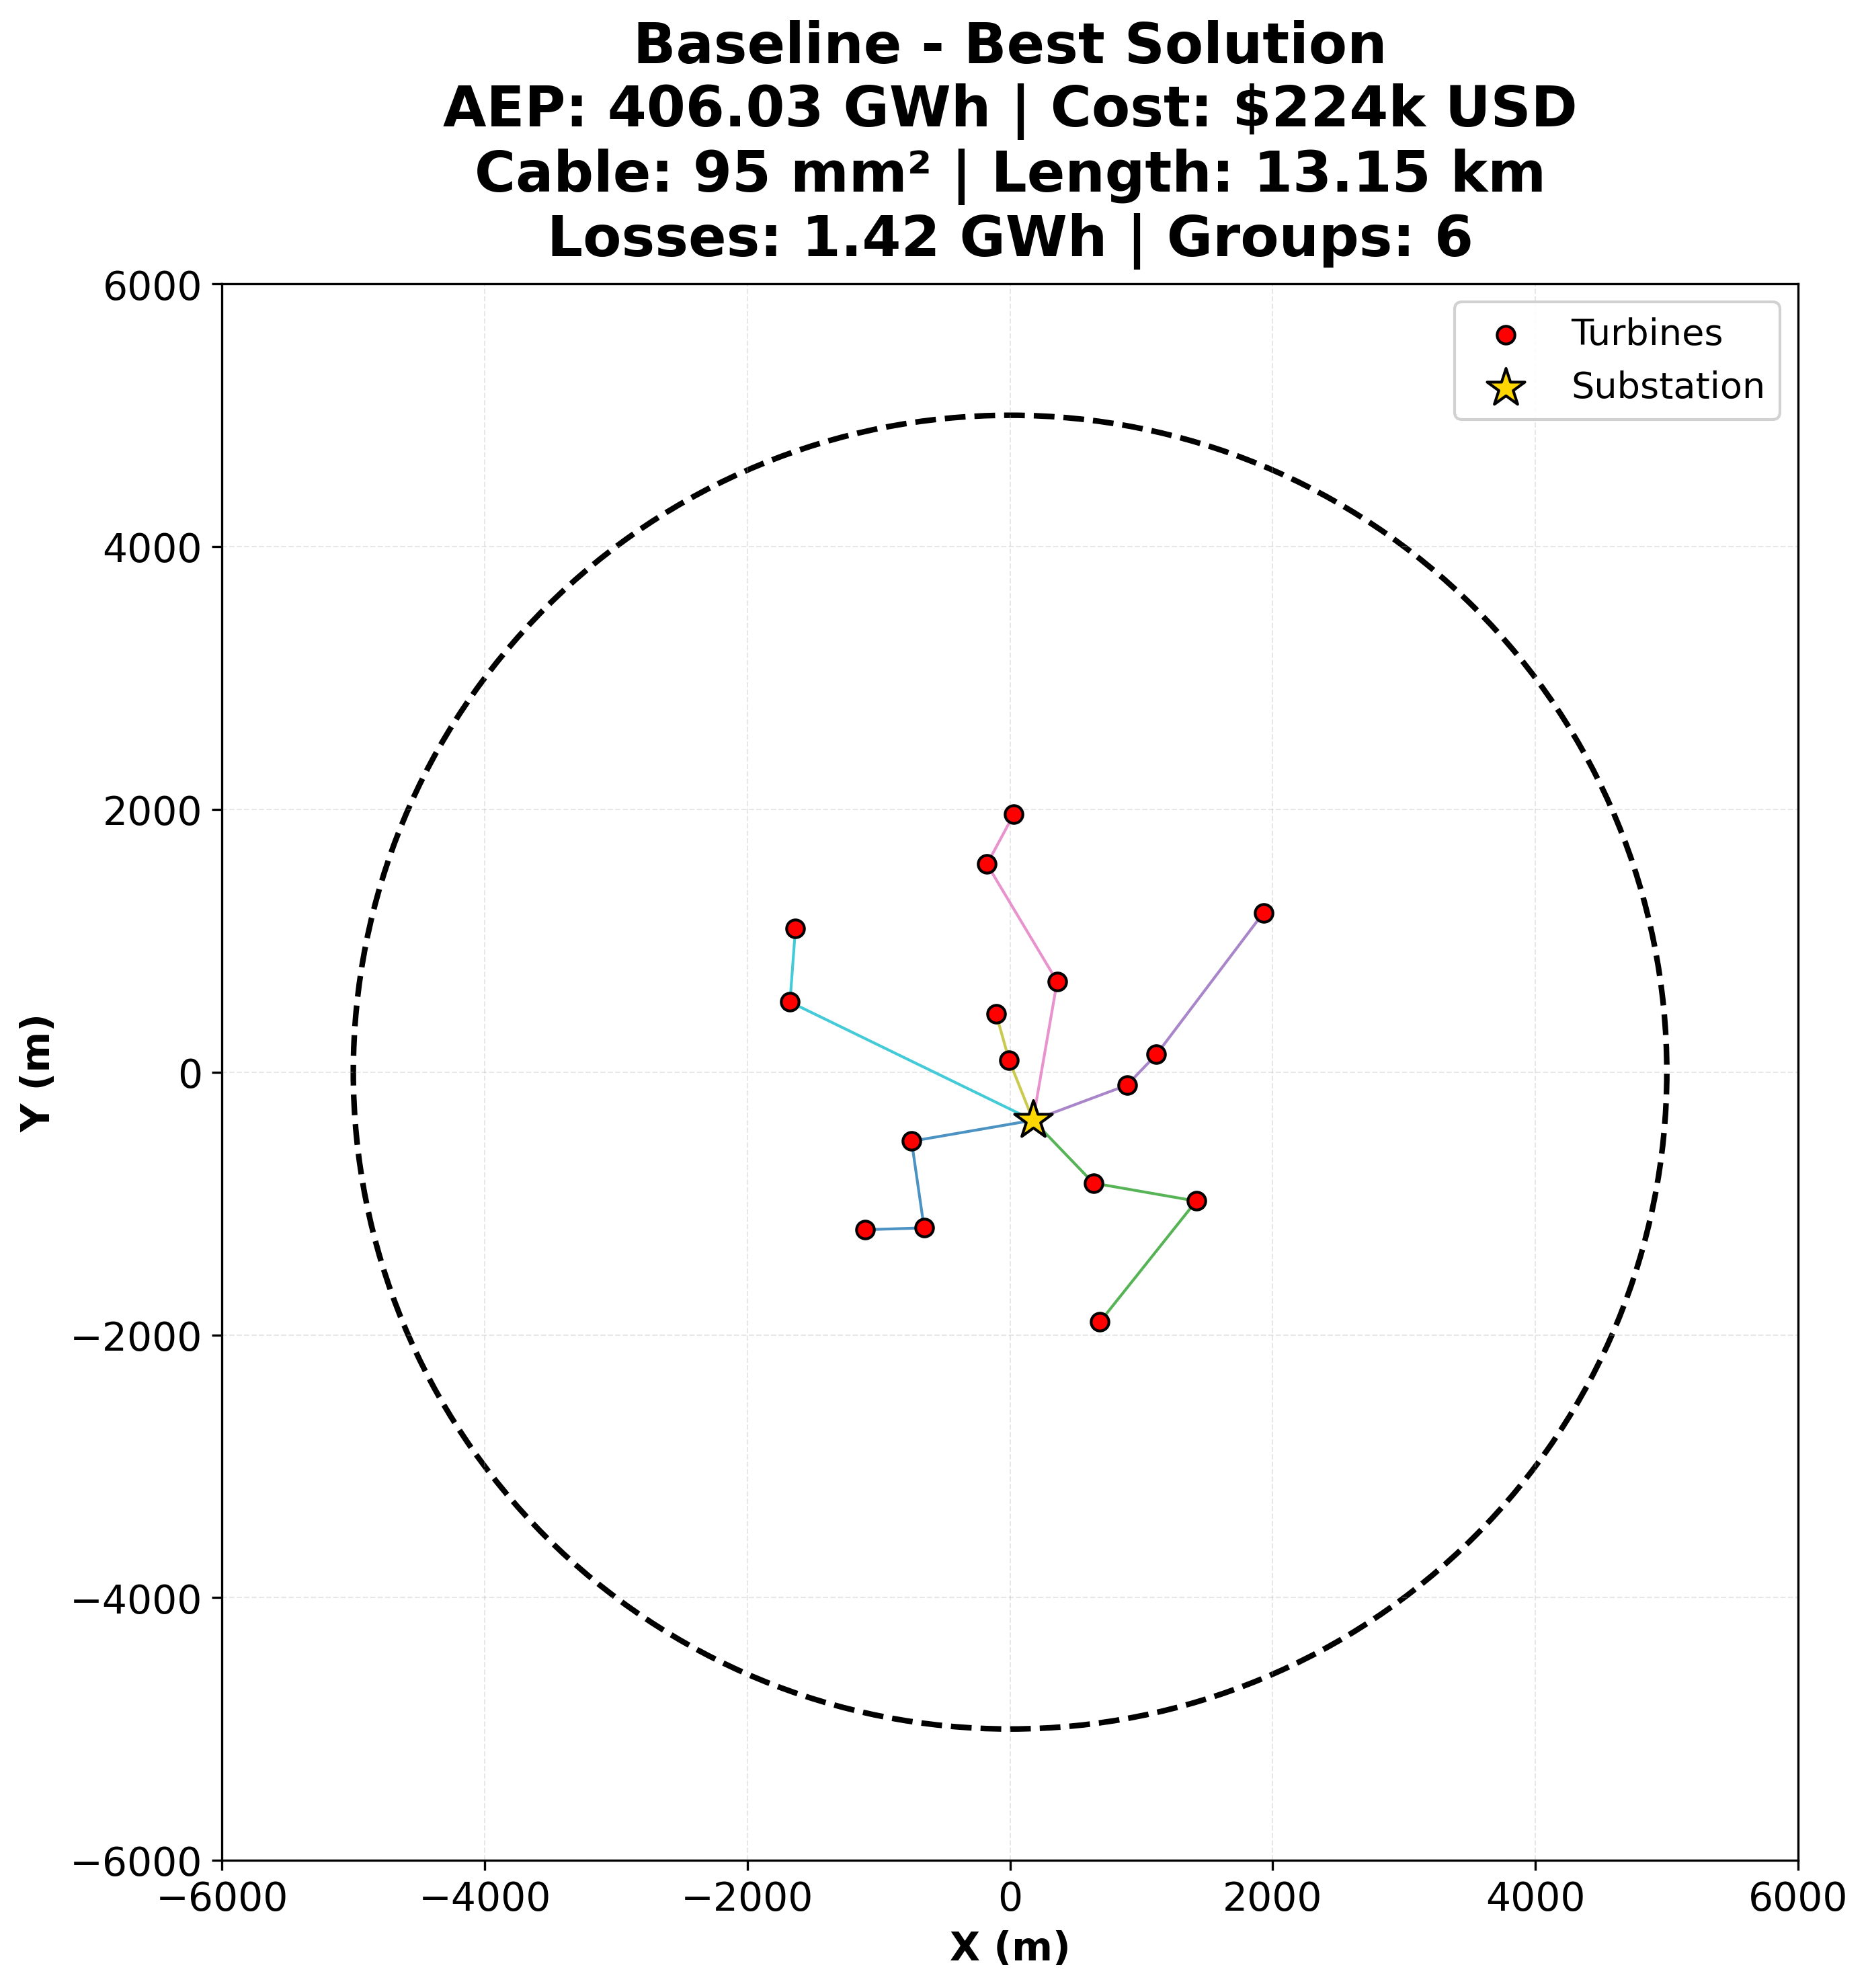
\includegraphics[width=\linewidth]{img/baseline_solution_16.png}
    \caption{Baseline}
    \label{fig:layout_16_baseline}
\end{subfigure}
\hfill
\begin{subfigure}[b]{0.33\textwidth}
    \centering
    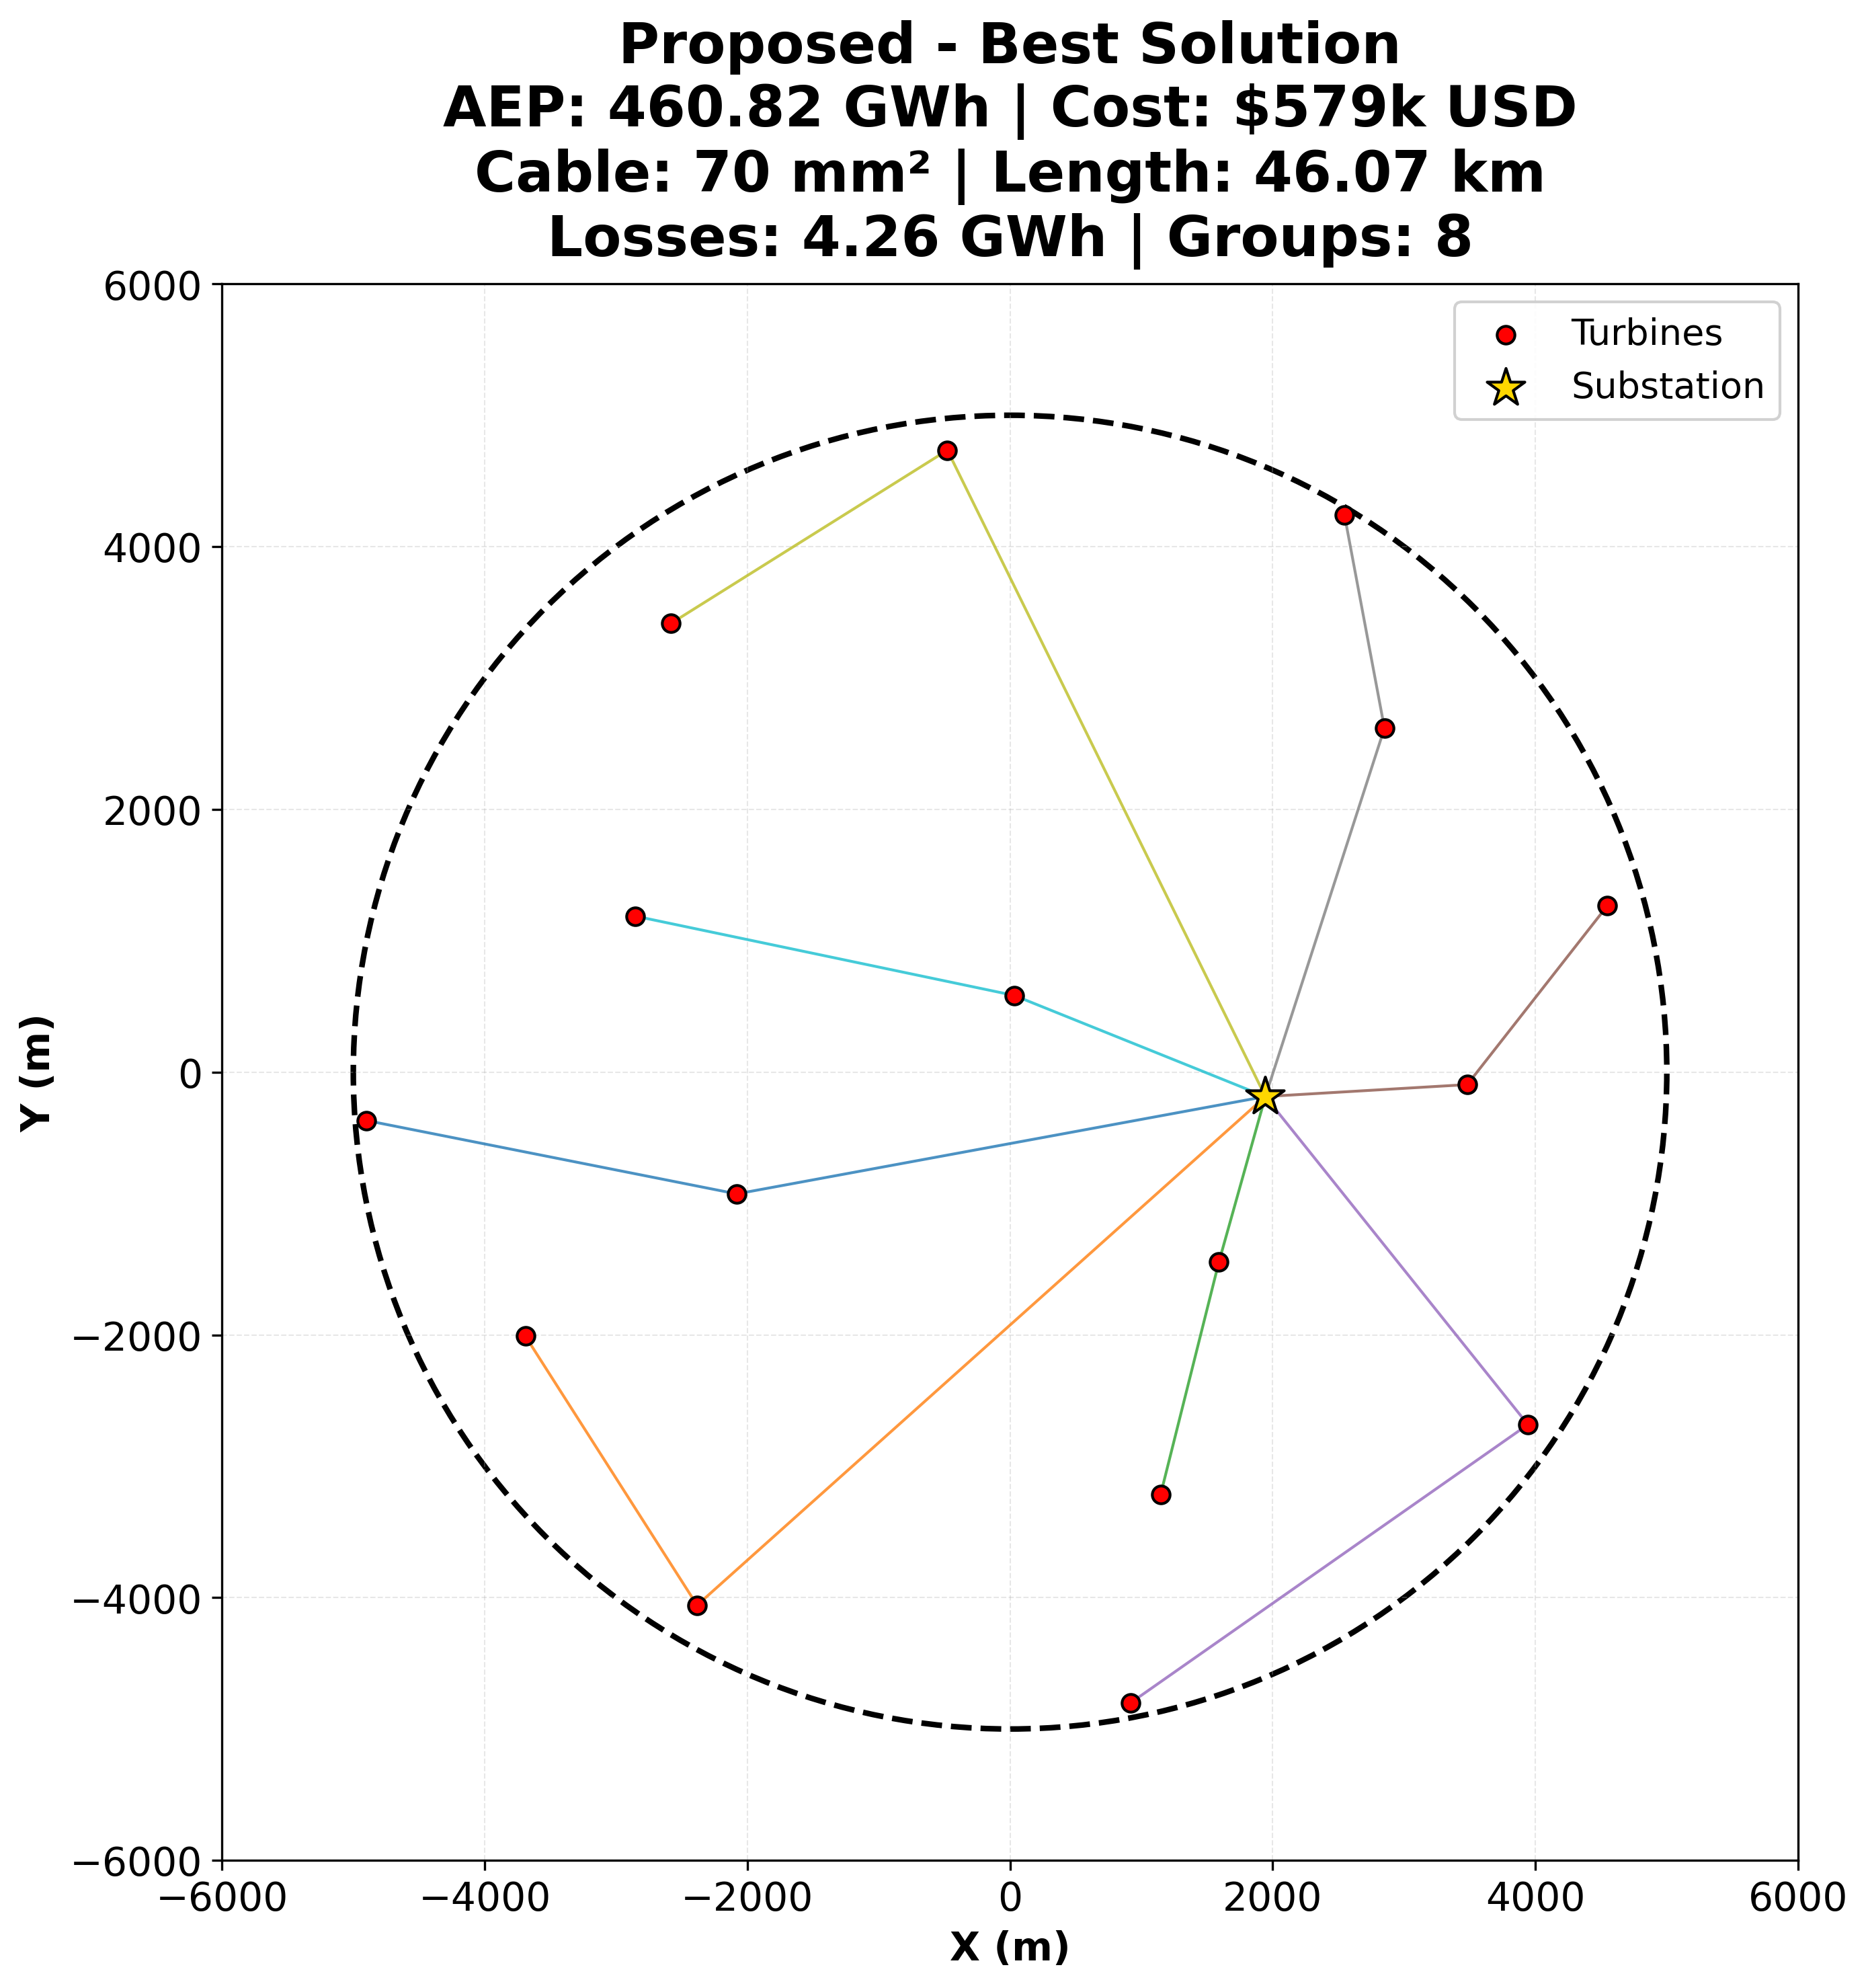
\includegraphics[width=\linewidth]{img/proposed_solution_16.png}
    \caption{Proposed}
    \label{fig:layout_16_proposed}
\end{subfigure}
\hfill
\begin{subfigure}[b]{0.33\textwidth}
    \centering
    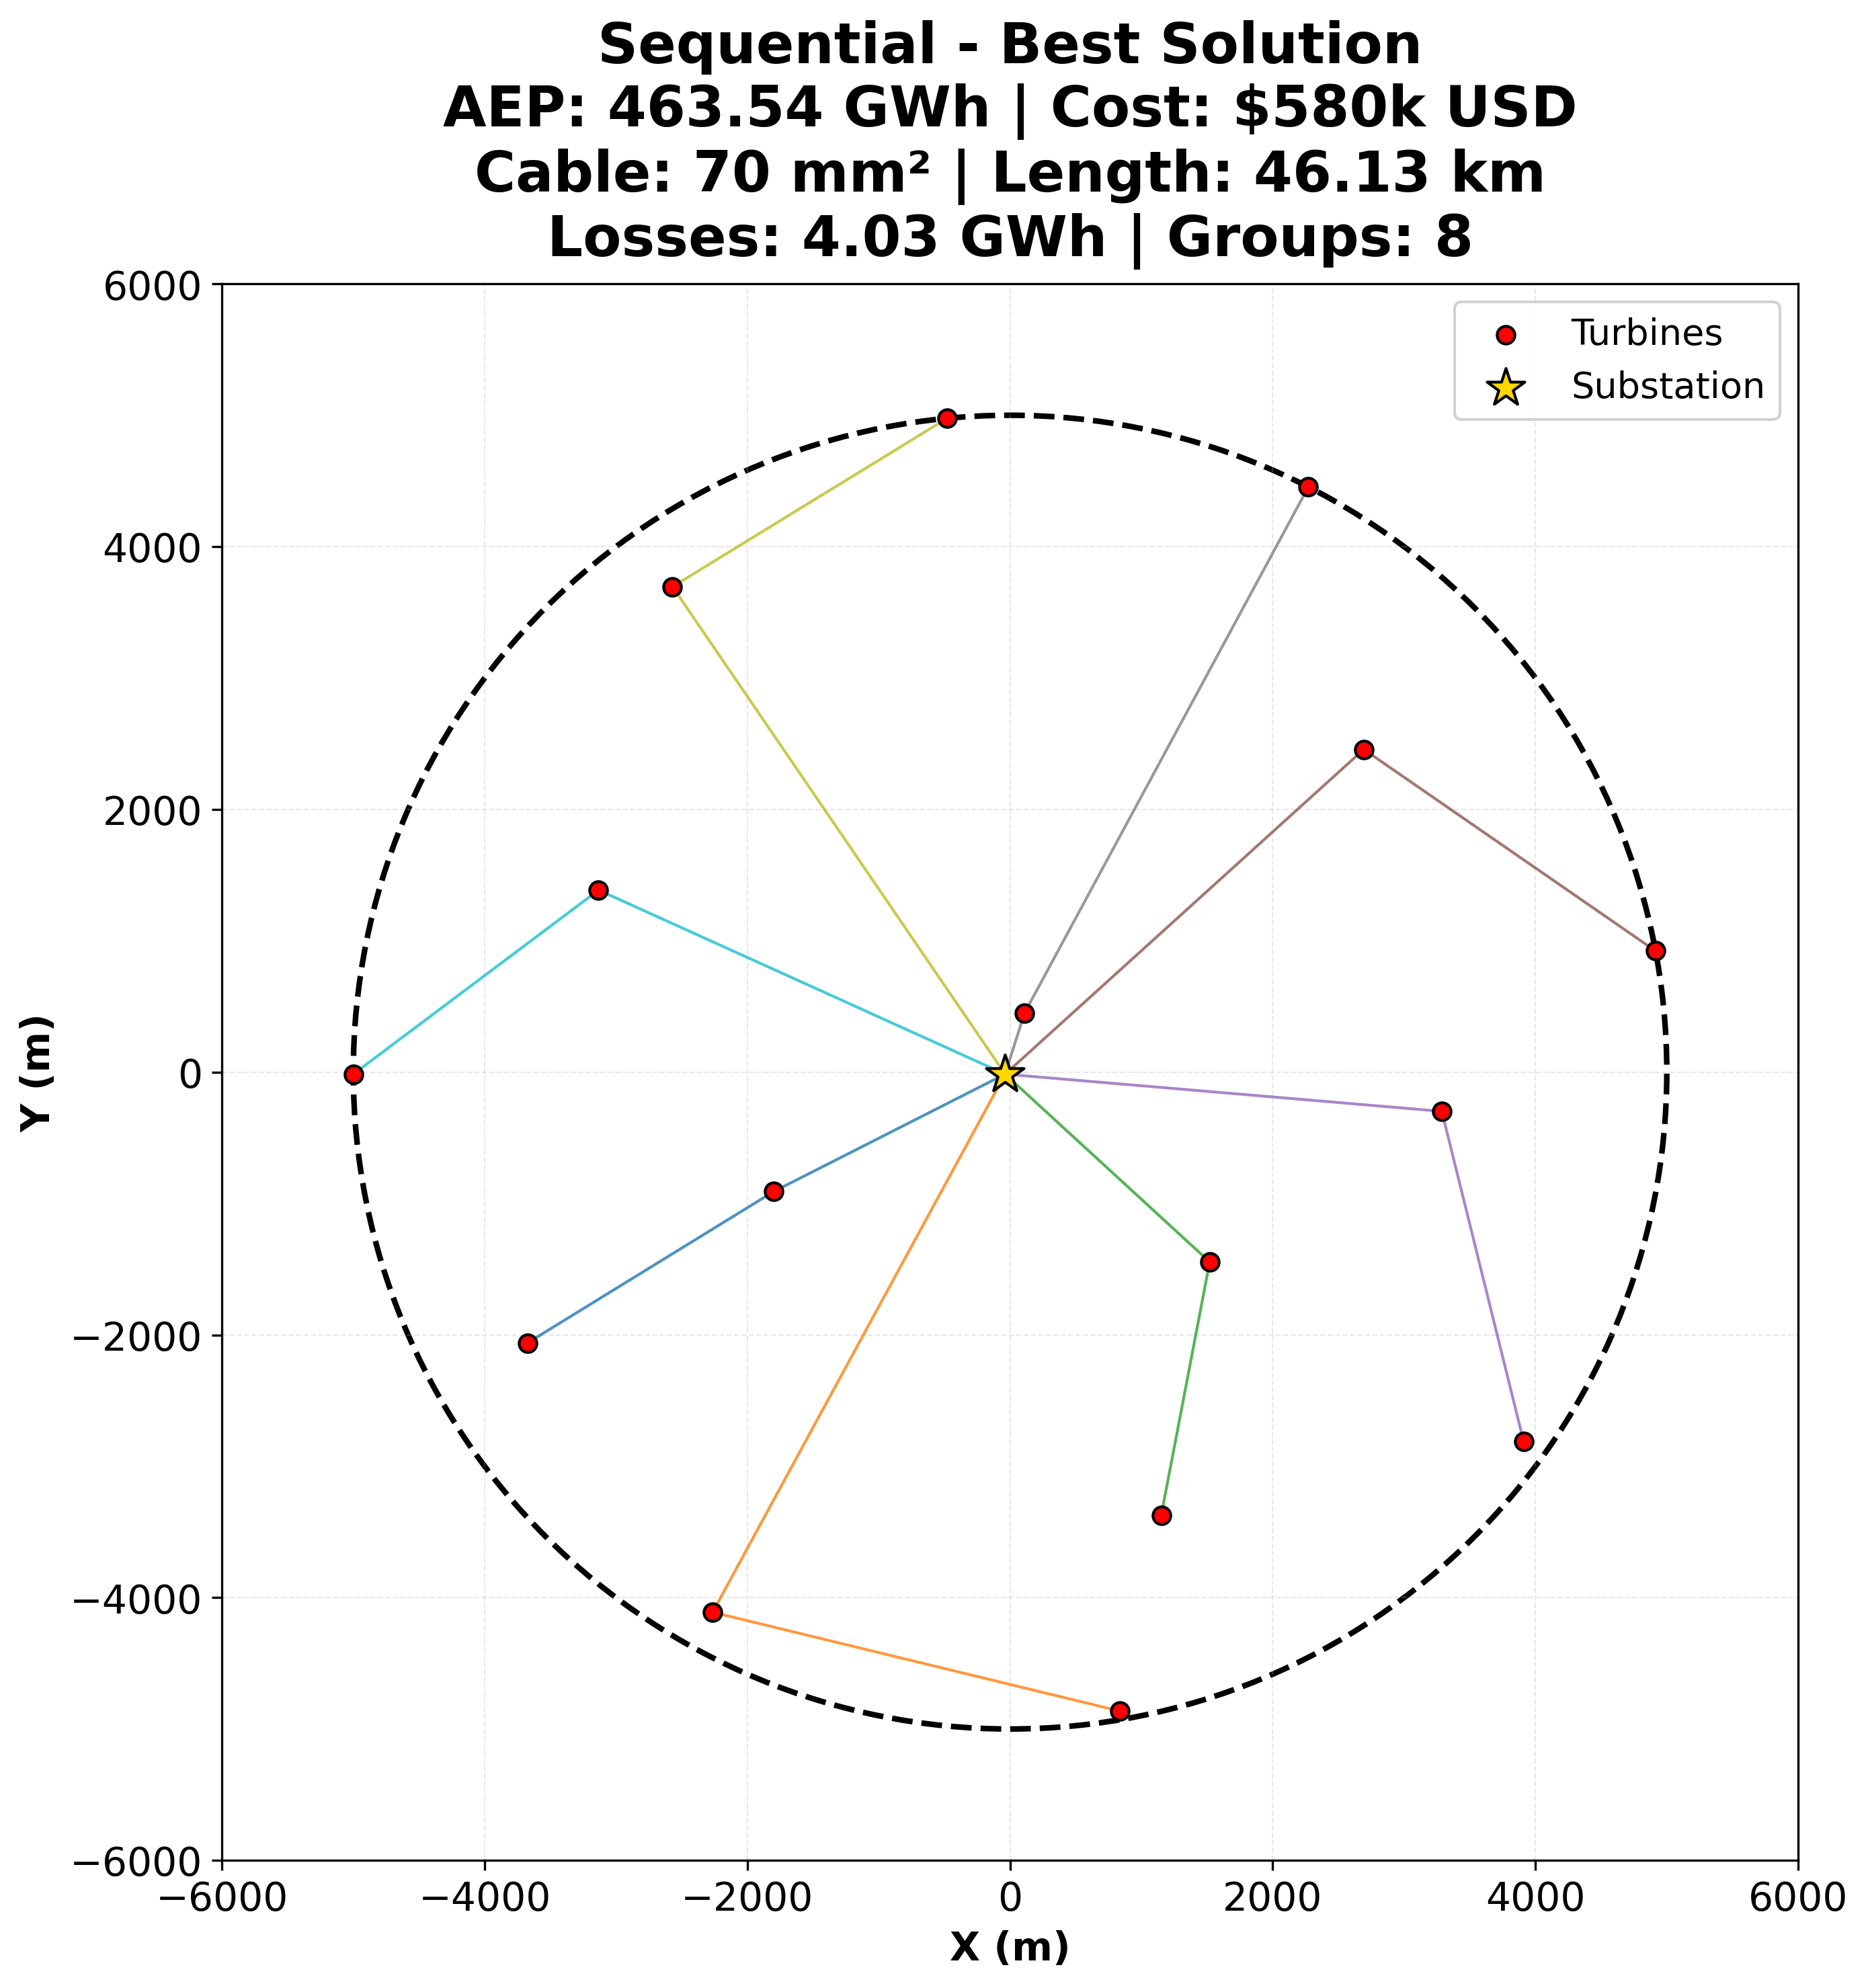
\includegraphics[width=\linewidth]{img/sequential_solution_16.png}
    \caption{Sequential}
    \label{fig:layout_16_sequential}
\end{subfigure}

\vspace{0.5cm}

% Linha 2: 36 Turbinas
\begin{subfigure}[b]{0.32\textwidth}
    \centering
    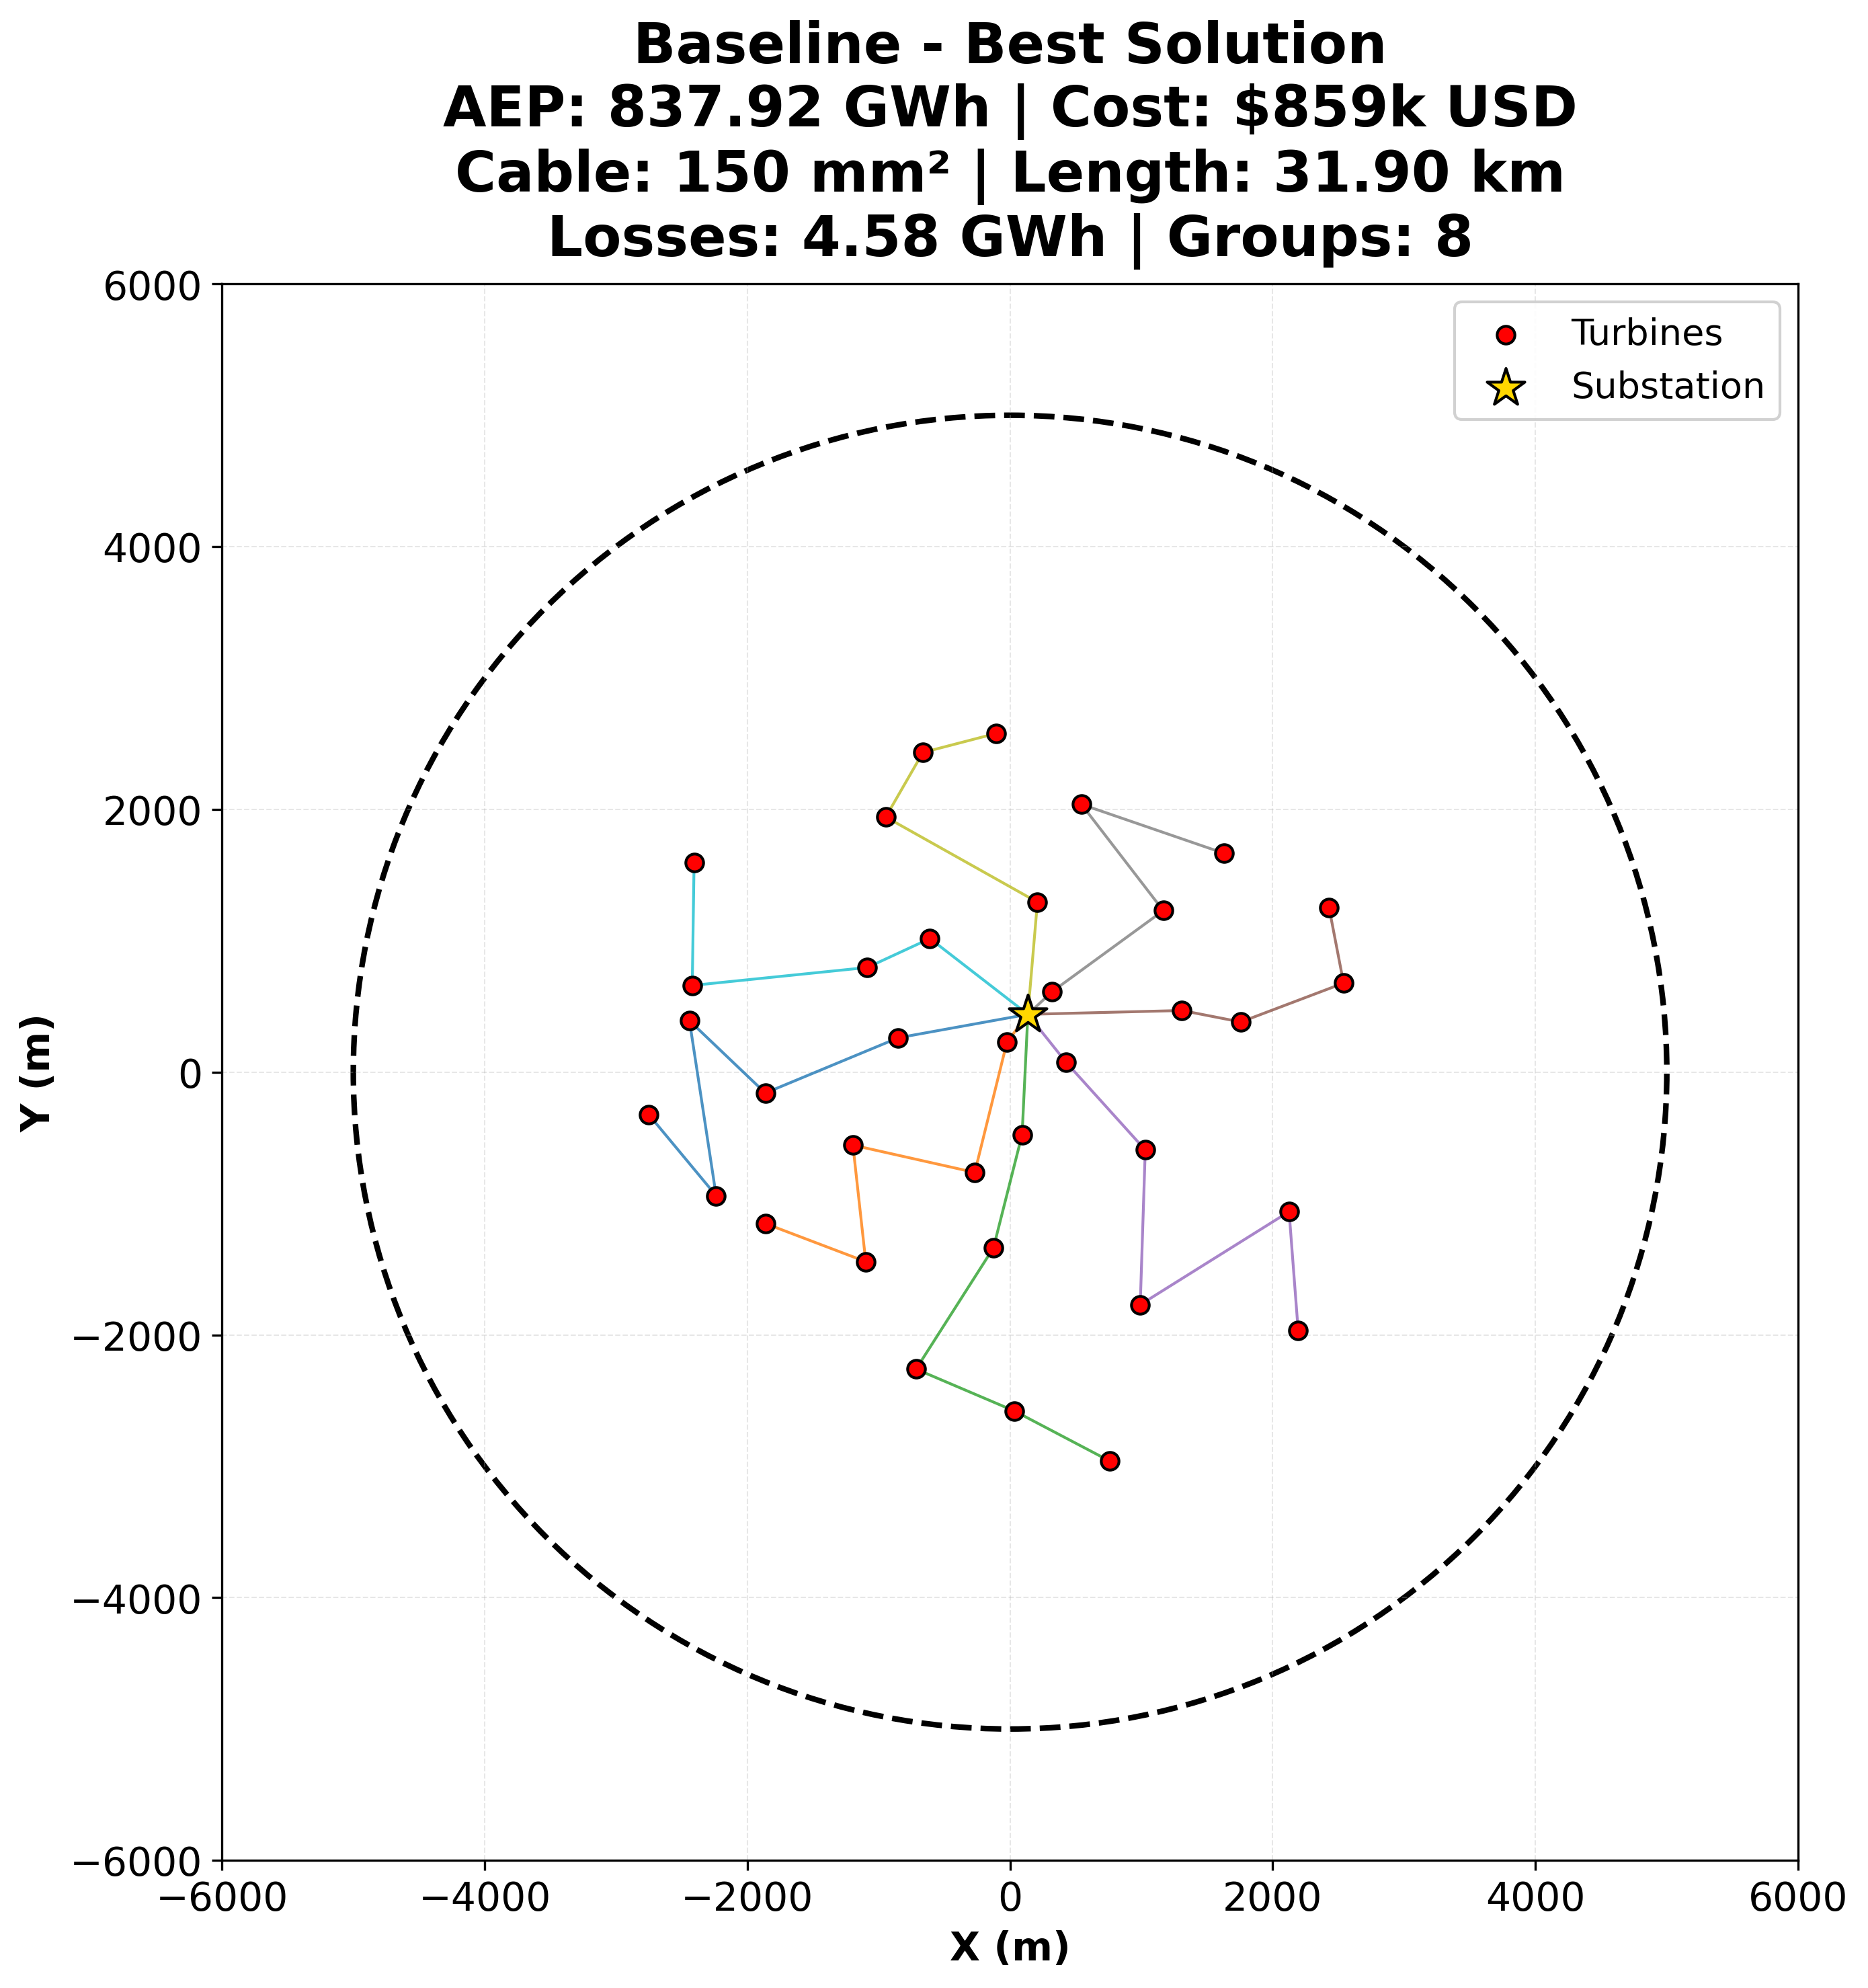
\includegraphics[width=\linewidth]{img/baseline_solution_36.png}
    \caption{Baseline}
    \label{fig:layout_36_baseline}
\end{subfigure}
\hfill
\begin{subfigure}[b]{0.32\textwidth}
    \centering
    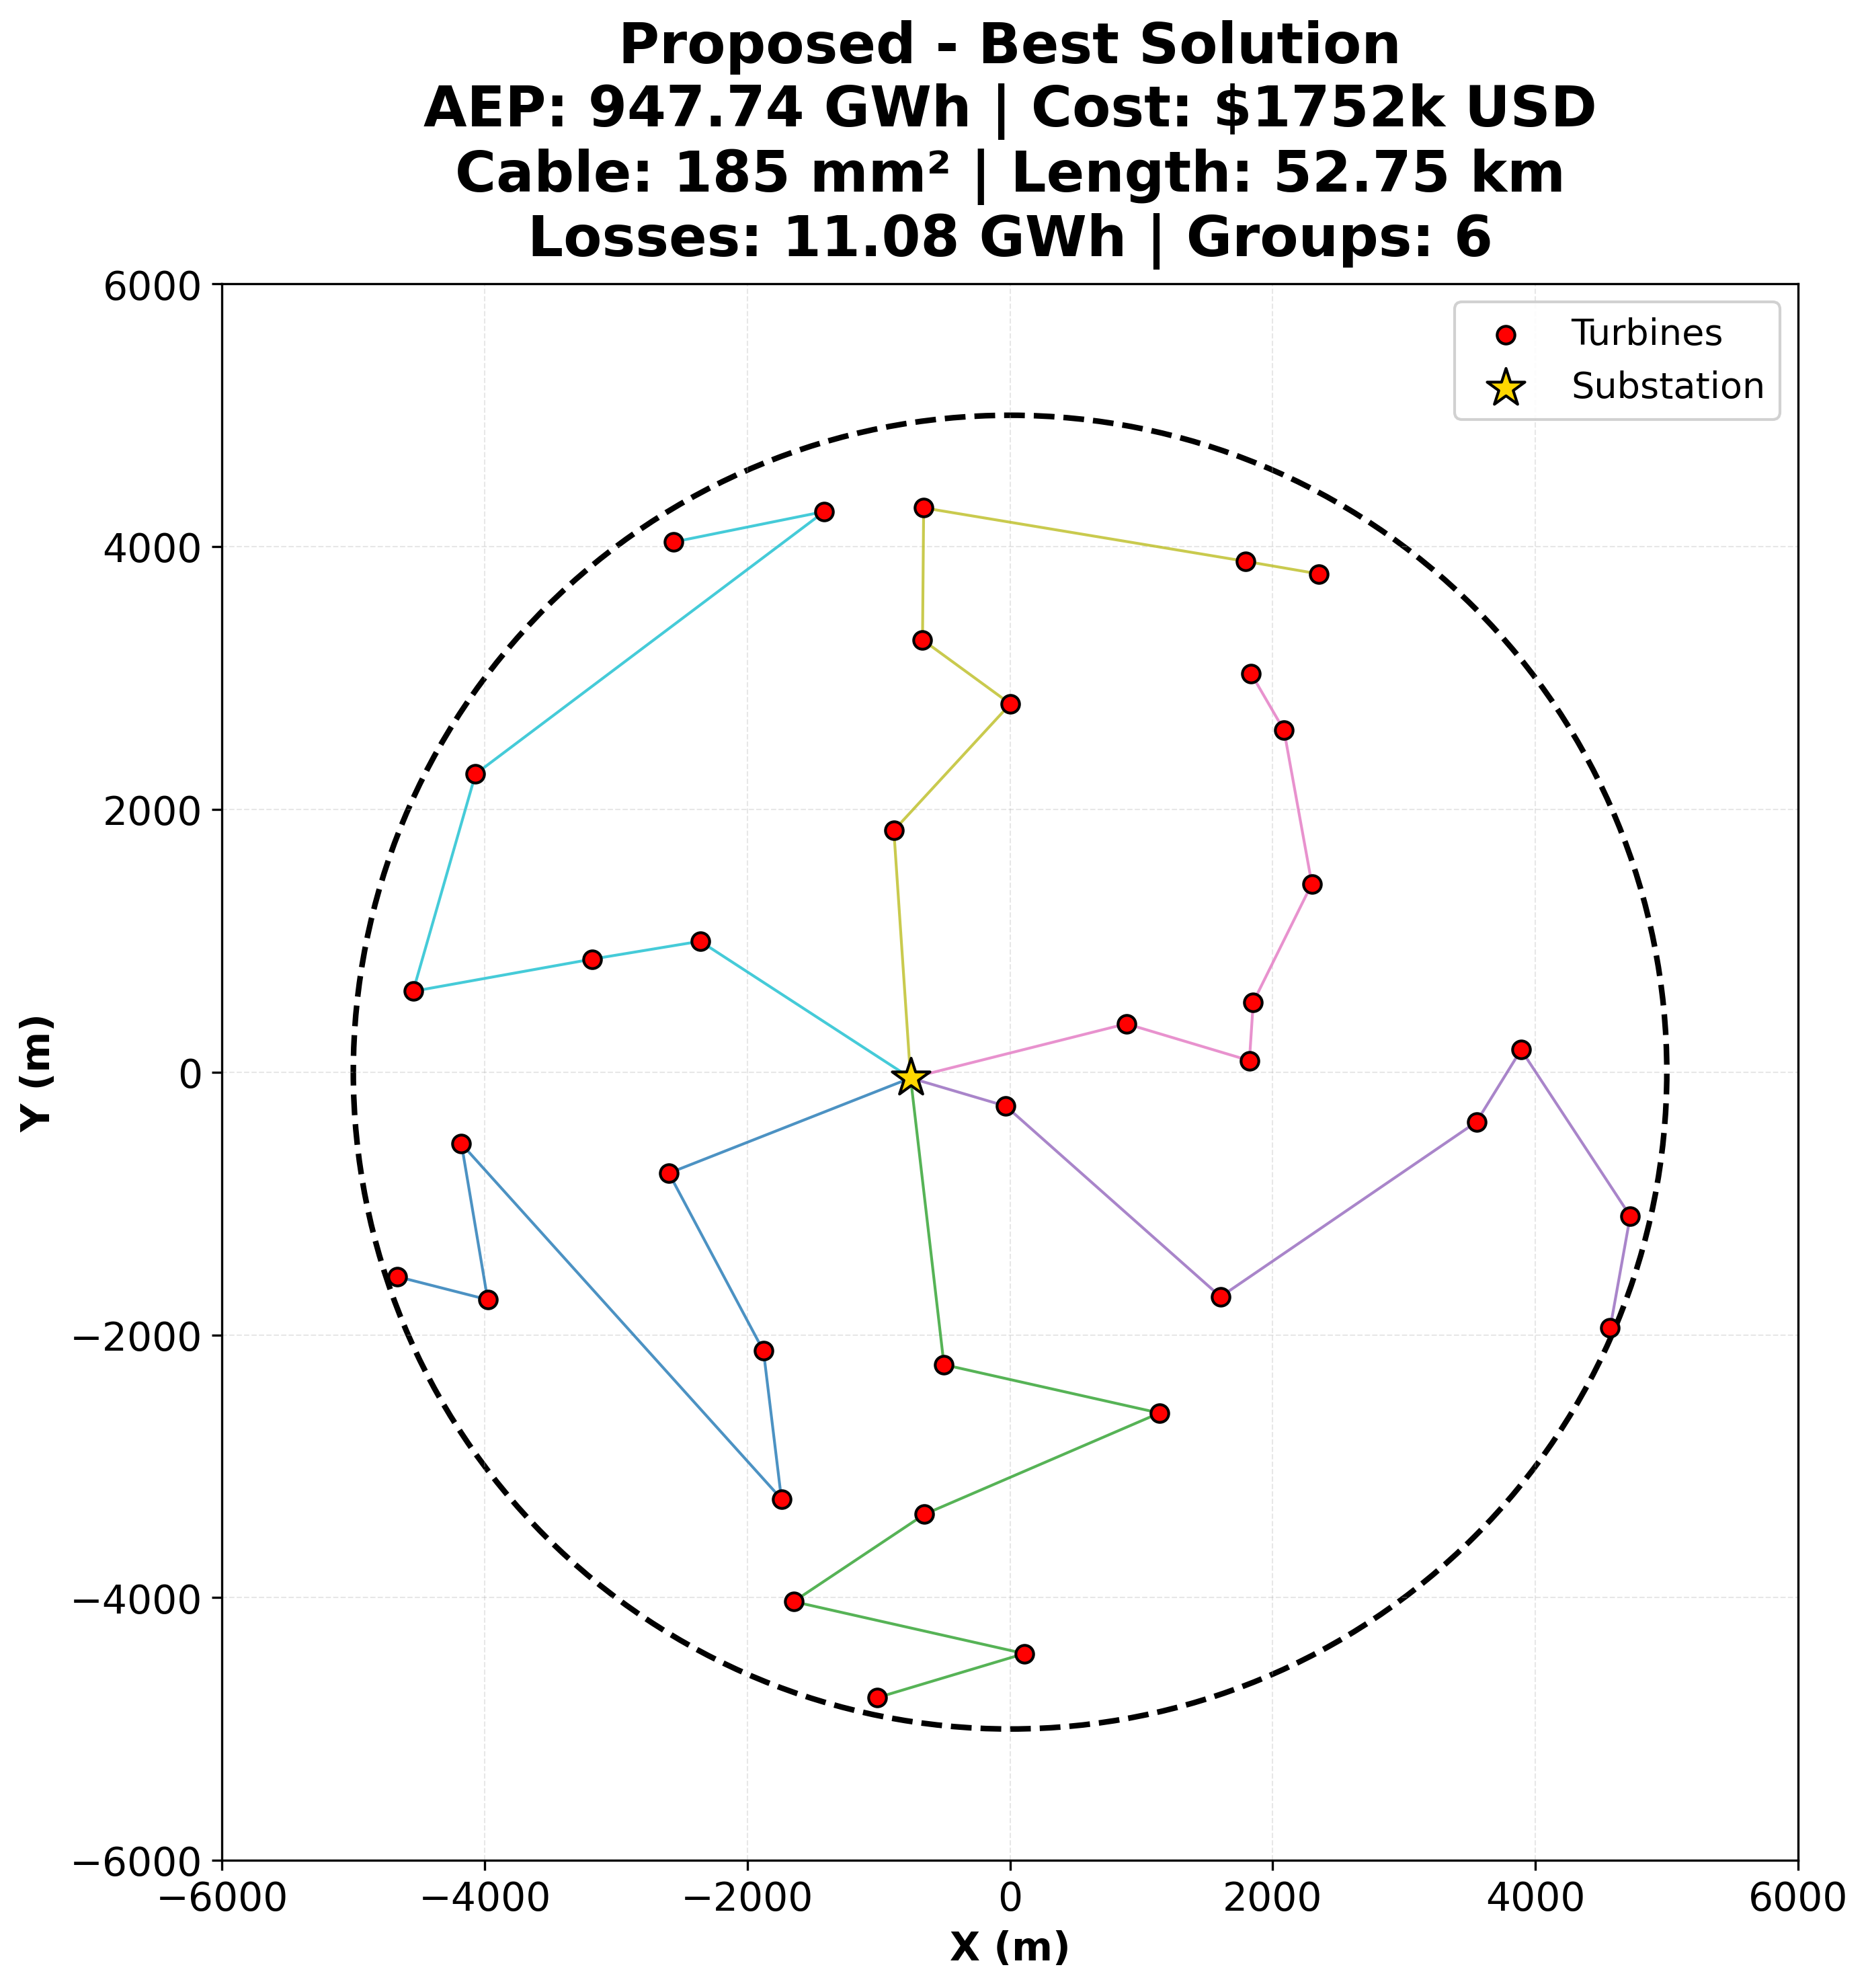
\includegraphics[width=\linewidth]{img/proposed_solution_36.png}
    \caption{Proposed}
    \label{fig:layout_36_proposed}
\end{subfigure}
\hfill
\begin{subfigure}[b]{0.32\textwidth}
    \centering
    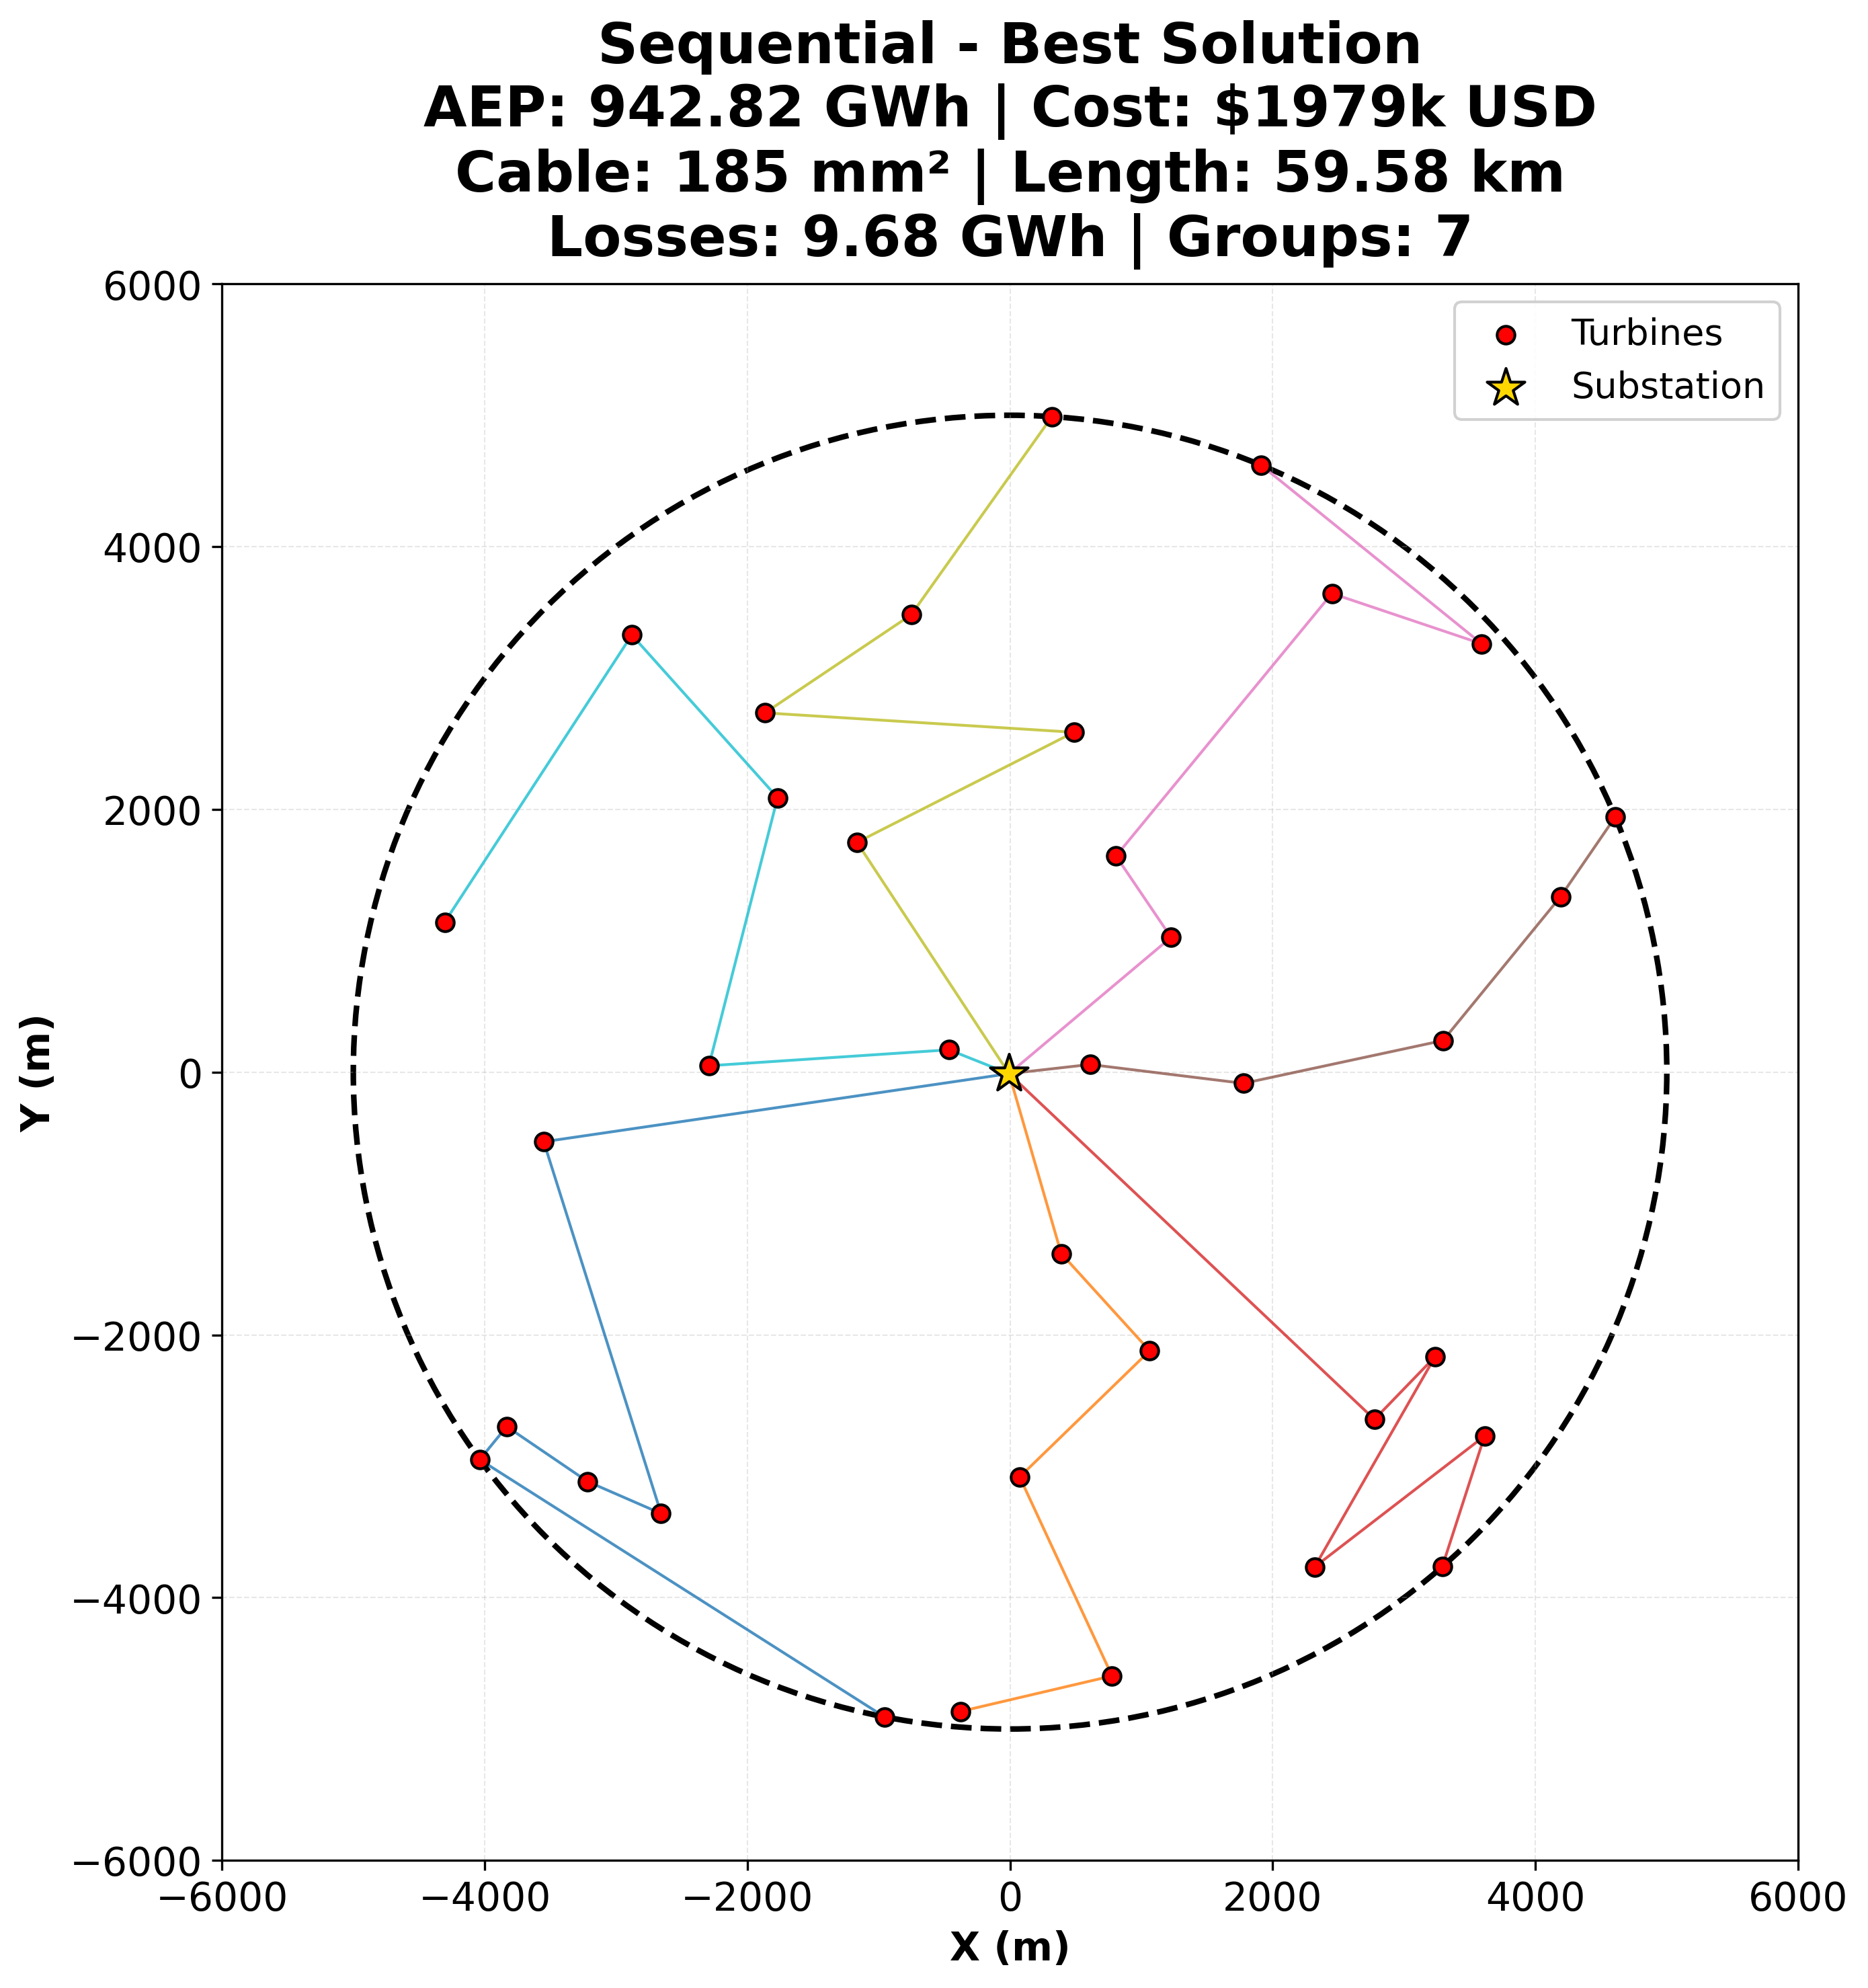
\includegraphics[width=\linewidth]{img/sequential_solution_36.png}
    \caption{Sequential}
    \label{fig:layout_36_sequential}
\end{subfigure}

\vspace{0.5cm}

% Linha 3: 64 Turbinas
\begin{subfigure}[b]{0.32\textwidth}
\centering
    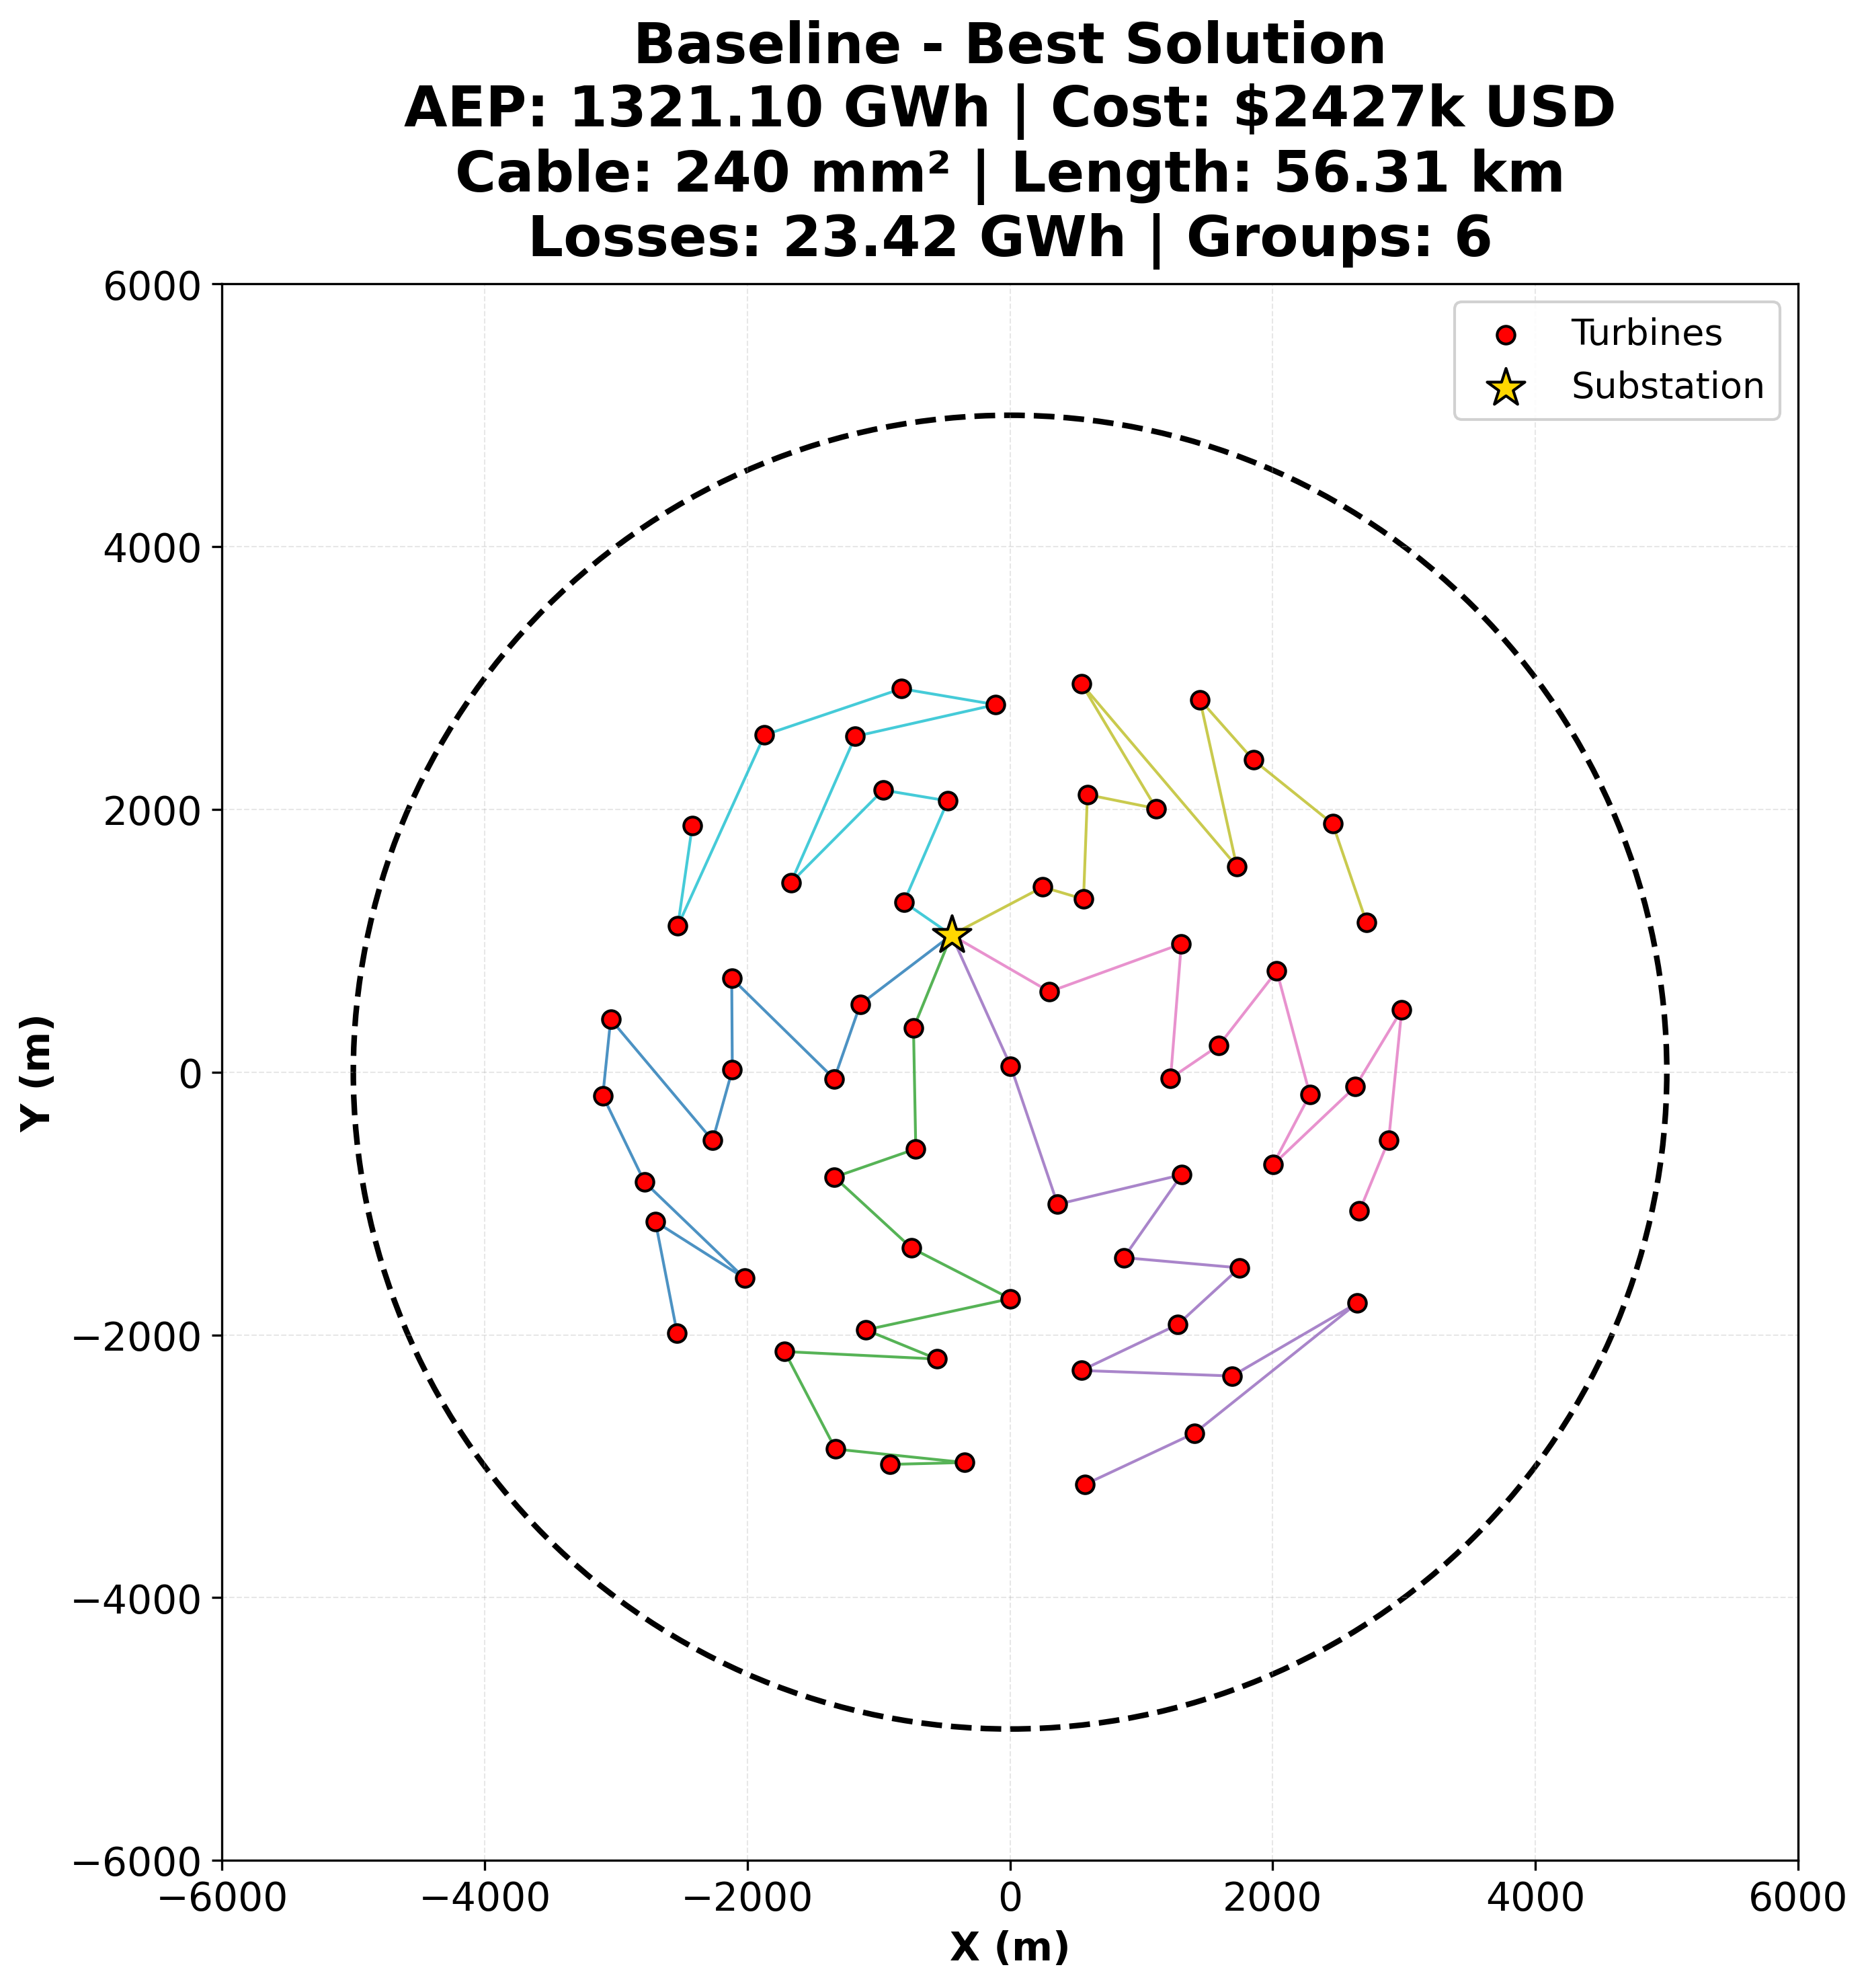
\includegraphics[width=\linewidth]{img/baseline_solution_64.png}
    \caption{Baseline}
    \label{fig:layout_64_baseline}
\end{subfigure}
\hfill
\begin{subfigure}[b]{0.32\textwidth}
    \centering
    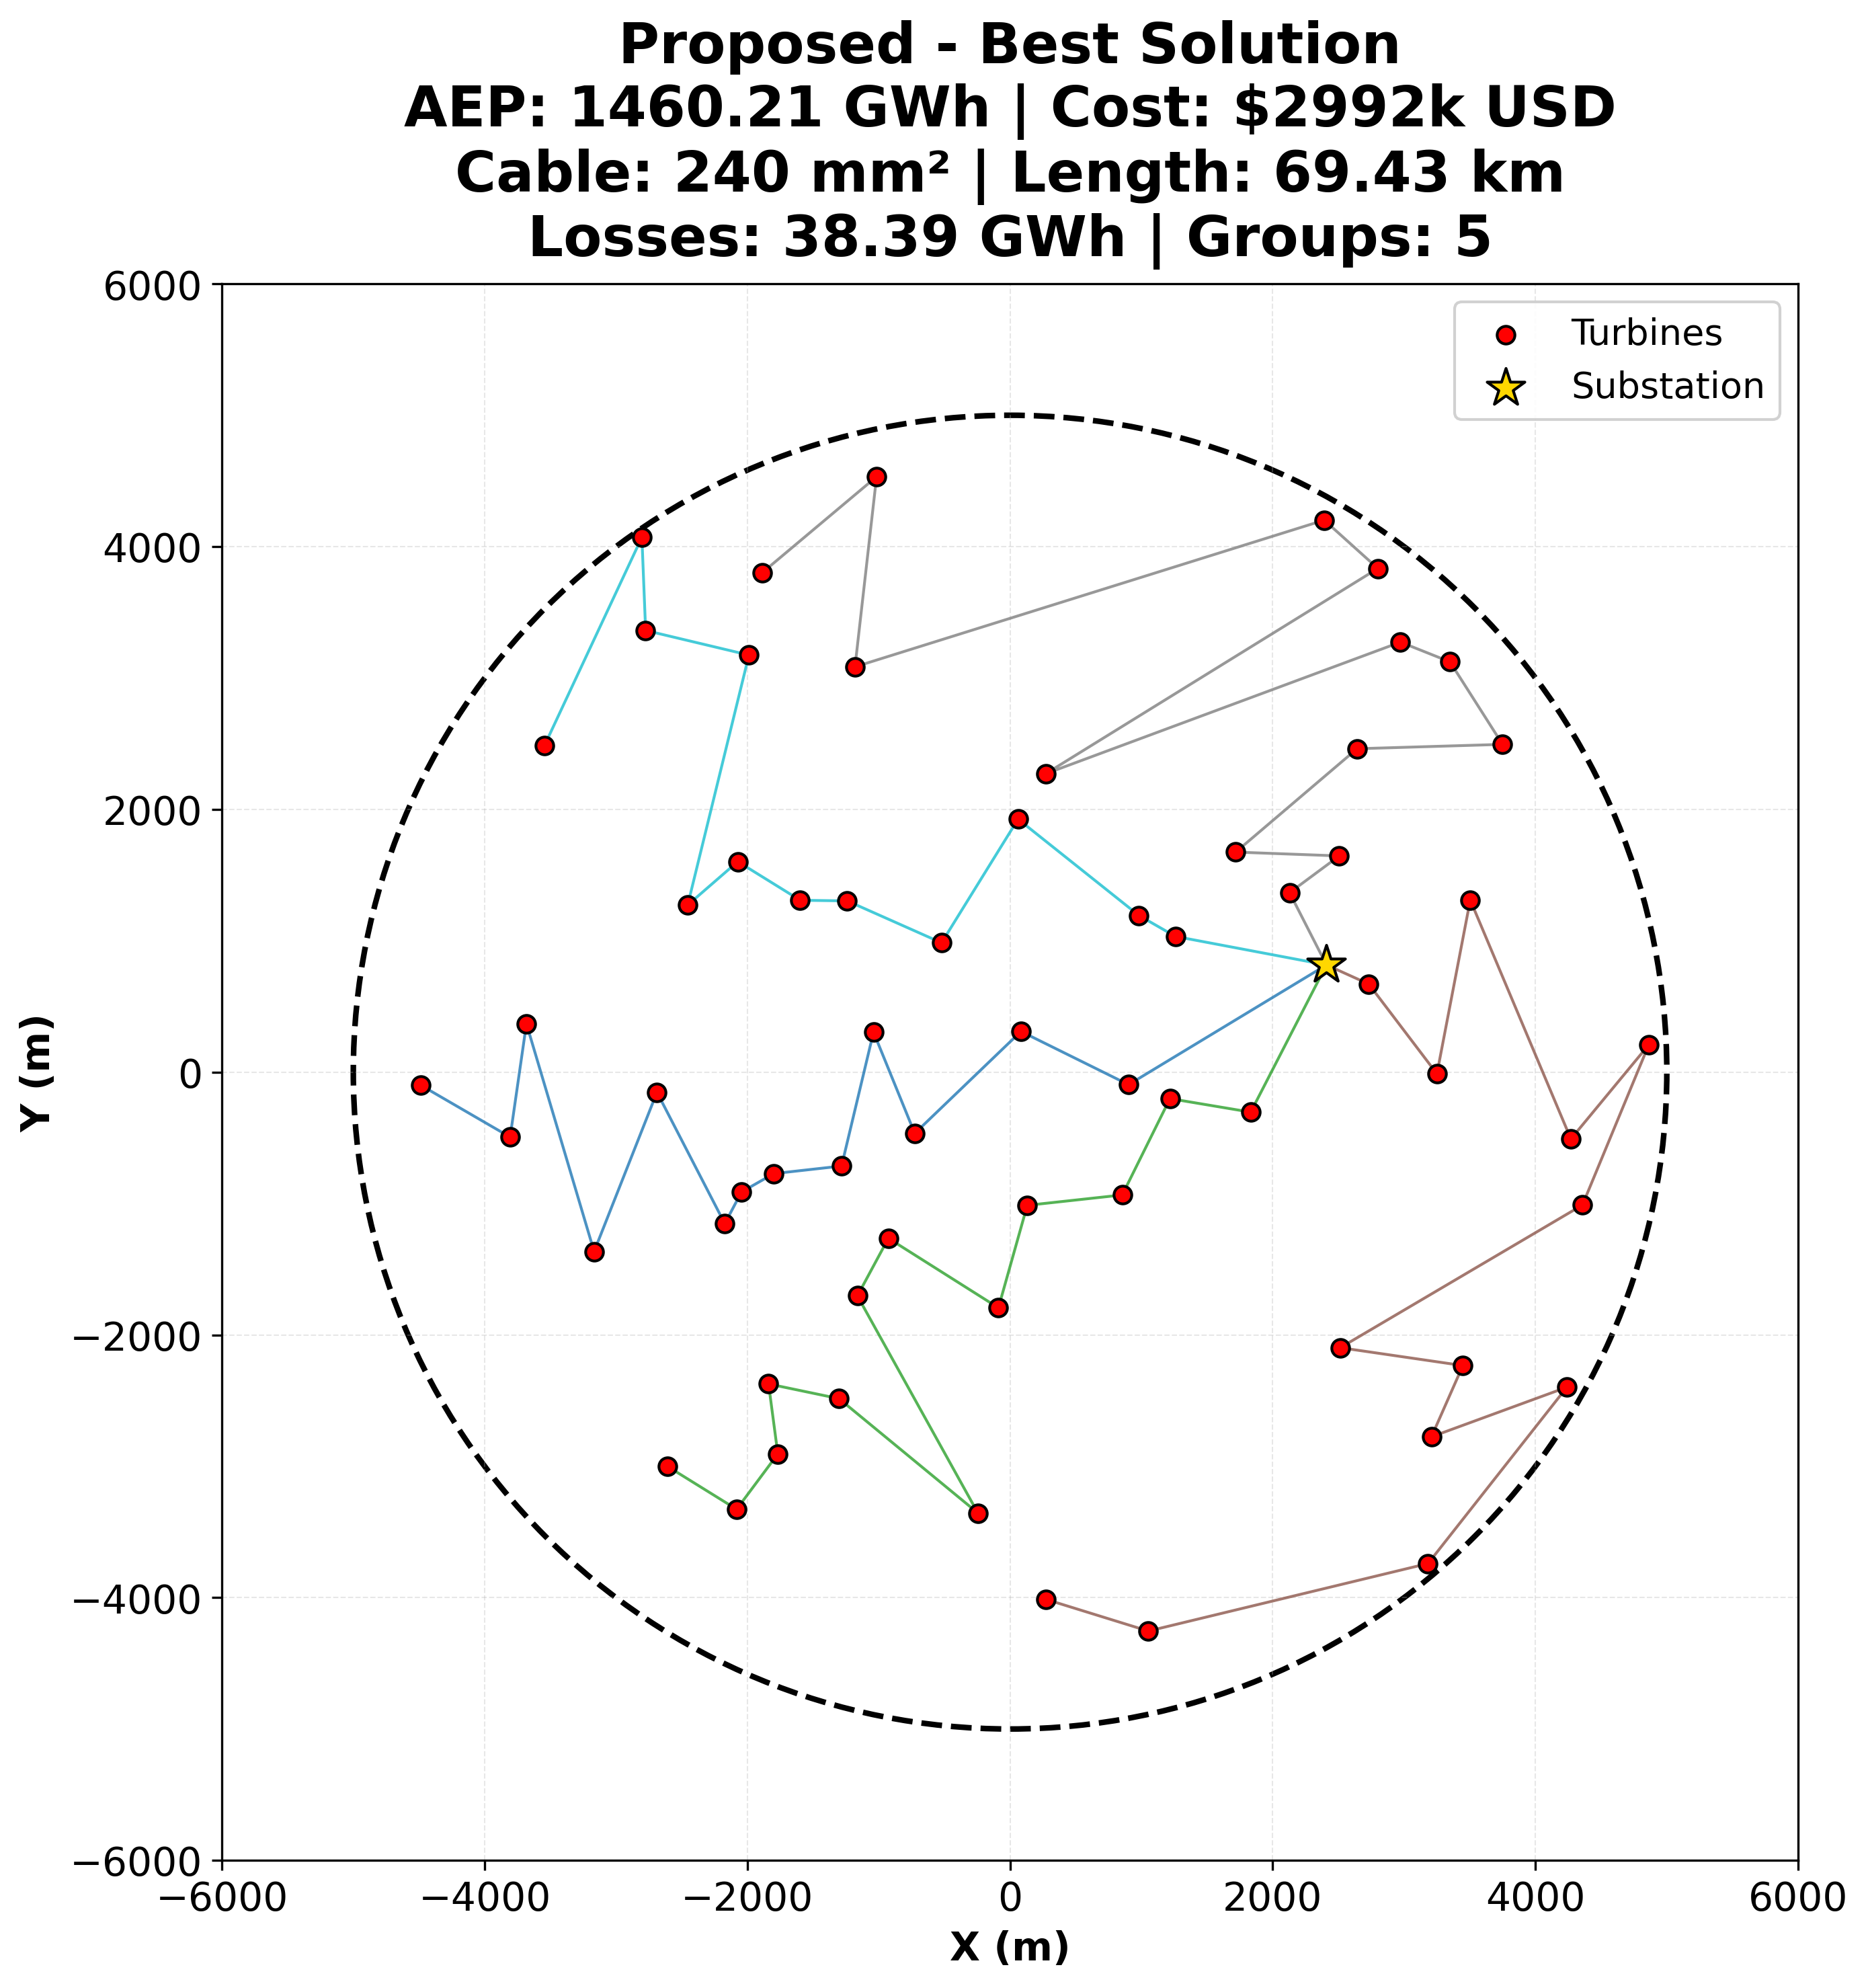
\includegraphics[width=\linewidth]{img/proposed_solution_64.png}
    \caption{Proposed}
    \label{fig:layout_64_proposed}
\end{subfigure}
\hfill
\begin{subfigure}[b]{0.32\textwidth}
    \centering
    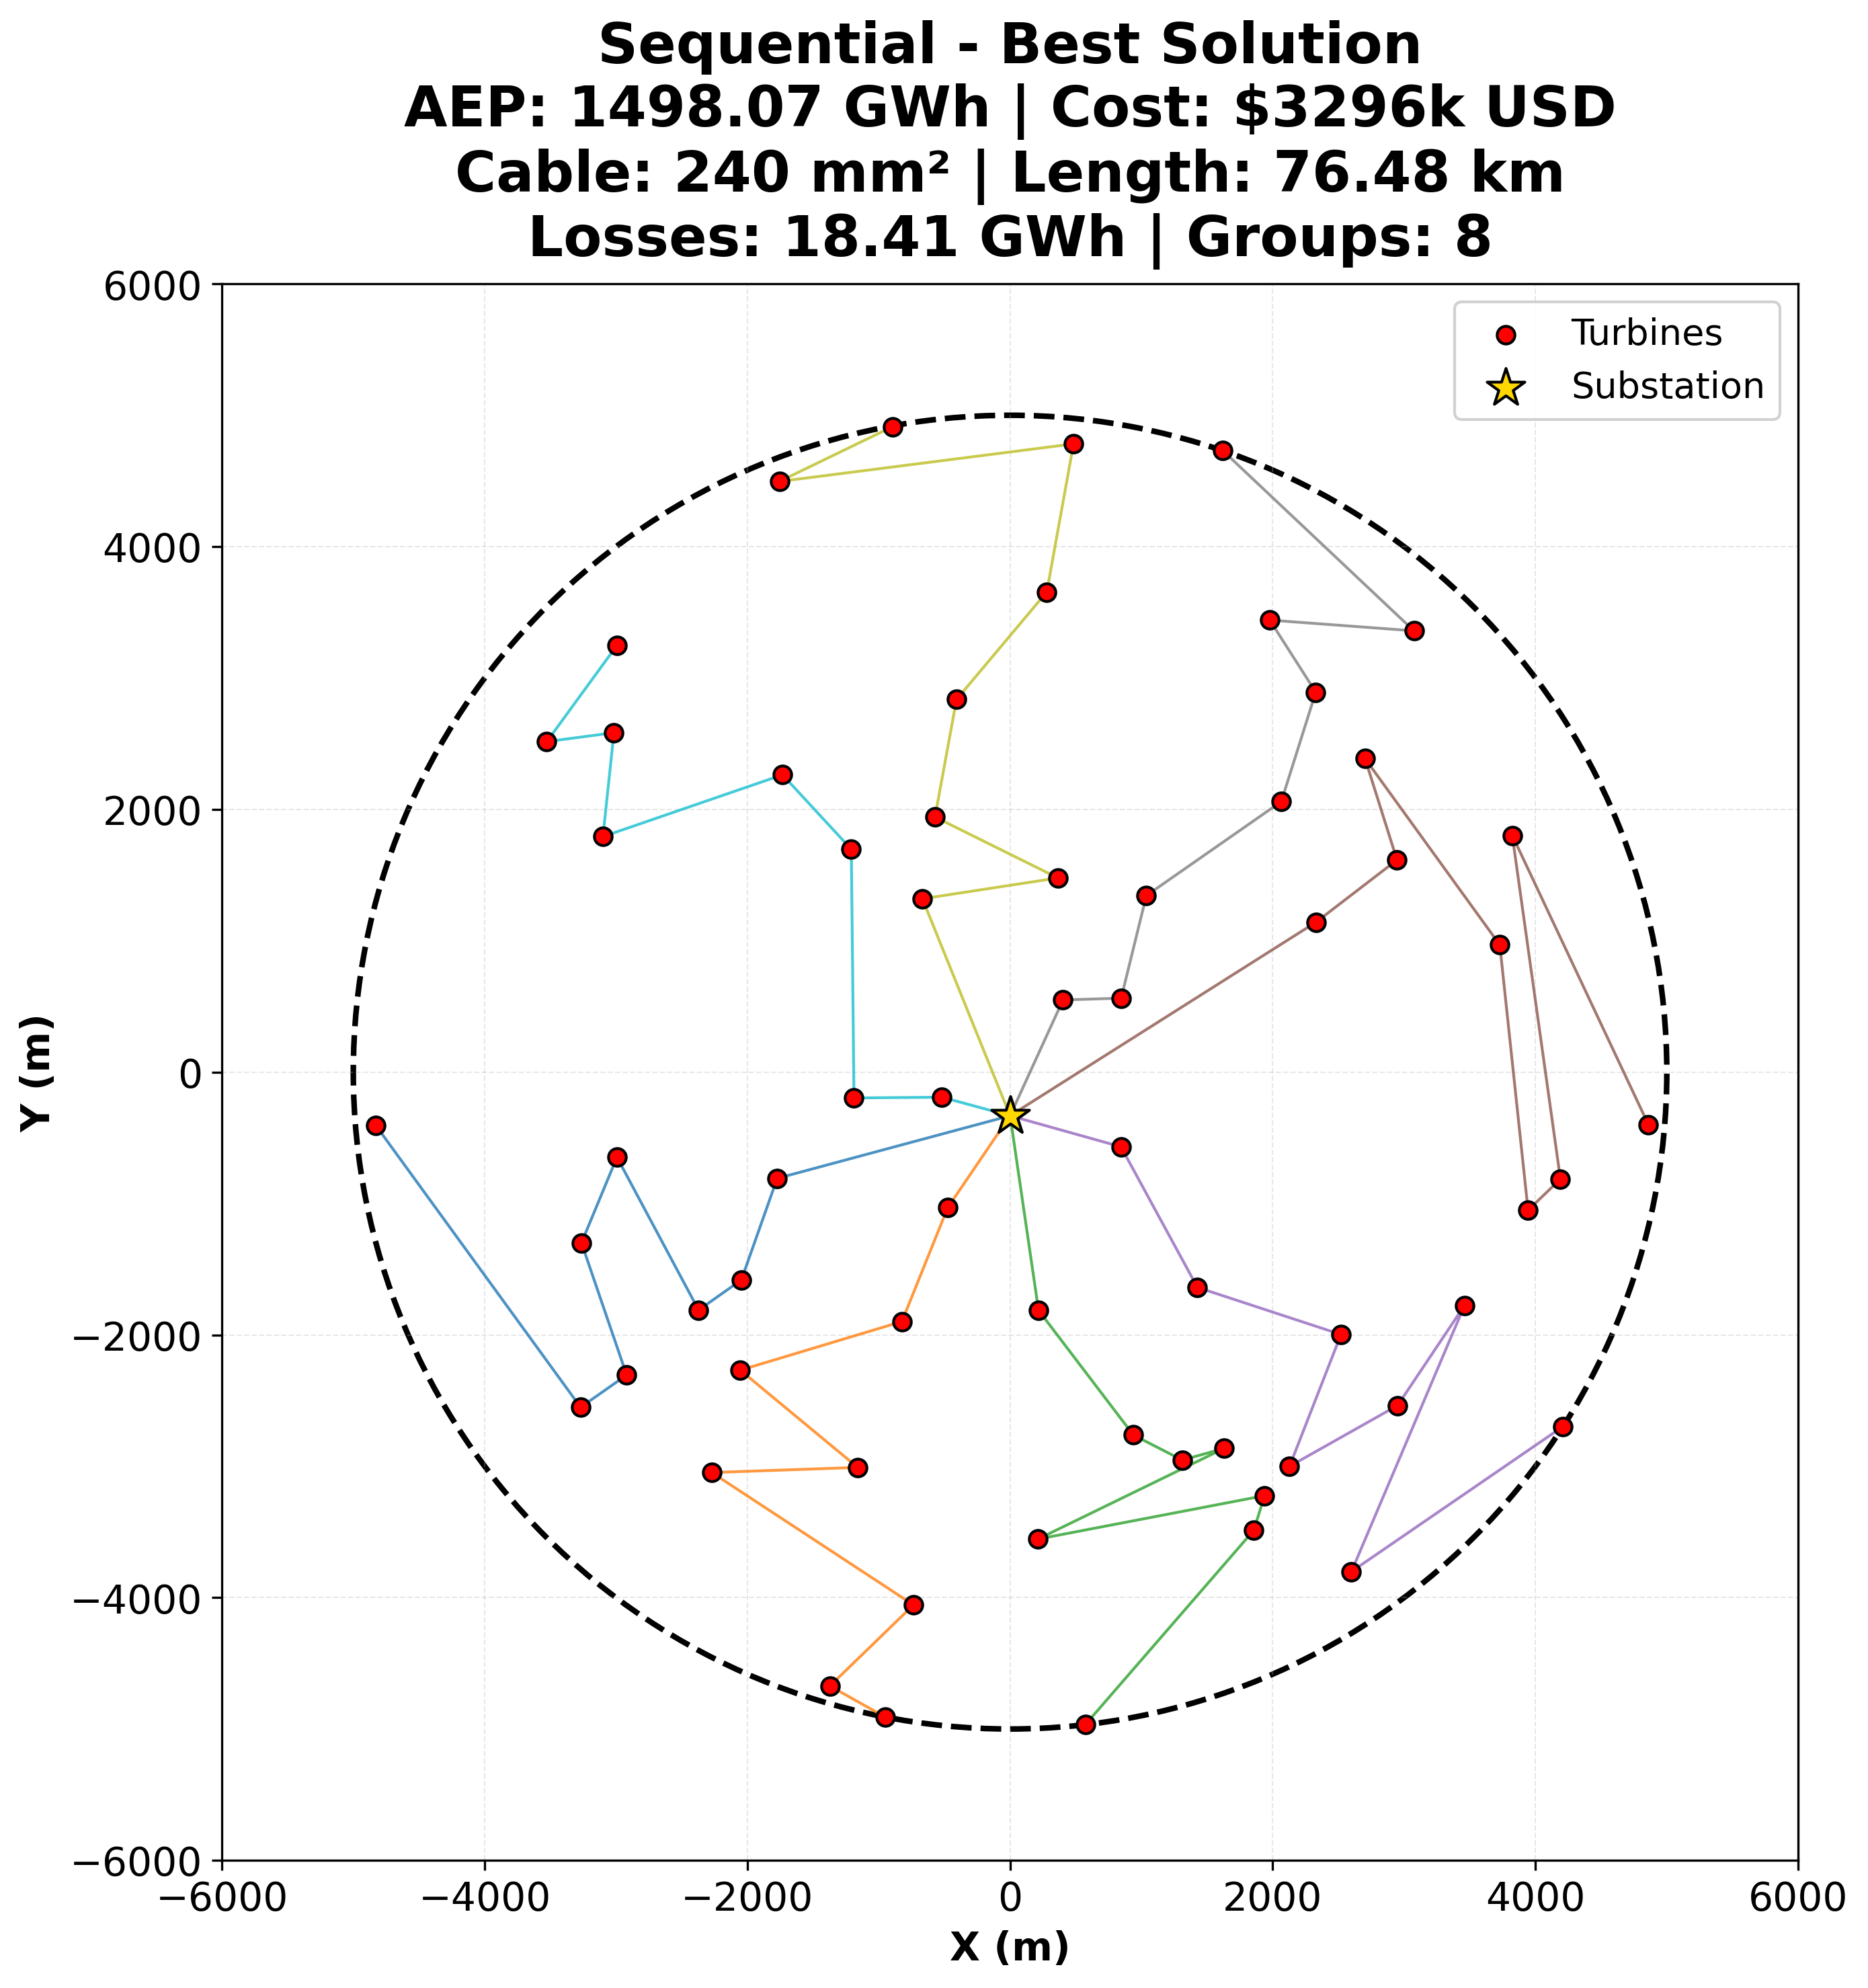
\includegraphics[width=\linewidth]{img/sequential_solution_64.png}
    \caption{Sequential}
    \label{fig:layout_64_sequential}
\end{subfigure}

\caption{Representative knee-point solutions across problem scales, obtained from a single representative run (one of 20 independent runs) for illustrative purposes. Top row: 16 turbines; middle row: 36 turbines; bottom row: 64 turbines. Columns represent Baseline, Proposed, and Sequential strategies, respectively. Colors denote cable strings generated by angular partitioning.}
\label{fig:layout_examples}
\end{figure*}

\subsection{Discussion and Limitations}

The comparative analysis is based on standardized IEA Task~37 benchmark scenarios \cite{Baker2019Best}, enabling controlled comparisons but omitting site-specific constraints (bathymetry, exclusion zones, port accessibility). The uniform cable section strategy reflects standard industrial practice for simplified procurement and installation.

The results demonstrate that hierarchical evolutionary strategies significantly enhance robustness and scalability across tested scales. At the largest scale (64 turbines), both Baseline and Proposed strategies exhibit seed-dependent hypervolume calculation issues, likely related to initialization difficulties in high-dimensional spaces (131 dimensions) rather than method-specific limitations. The Proposed framework maintains valid hypervolume for approximately half of the runs, while Baseline shows issues for all runs, highlighting the importance of initialization strategies for industrial-scale applications.

The comparison is restricted to NSGA-II; alternative evolutionary paradigms (e.g., MOEA/D, SPEA2) may exhibit different scalability characteristics. Future work will extend the framework to site-dependent constraints. Additionally, improved cable group initialization strategies should be investigated, as random initialization within the full range (e.g., 5--64 groups for 64 turbines) may not be optimal. Geometric constraints suggest that initializing with group counts that better match the spatial distribution of turbines could improve convergence reliability, particularly at larger scales where few groups (see Table~\ref{tab:qualitative_characteristics} for group count statistics) may create routing difficulties without cable crossings.

%
\section{Conclusion}

This paper investigated how different evolutionary optimization strategies influence the quality, scalability, and robustness of integrated offshore wind farm design through a systematic comparison of three paradigms: fully coupled single-phase NSGA-II, sequential layout--infrastructure optimization, and a hierarchical two-phase evolutionary framework.

The results demonstrate that the optimization strategy plays a decisive role in resolving trade-offs between aerodynamic performance and electrical infrastructure cost. The Sequential approach collapses to single solutions due to fixed-layout assumptions, while Baseline NSGA-II exhibits degraded convergence as dimensionality increases. In contrast, the proposed two-phase framework achieves stable, well-distributed Pareto fronts across all tested scales (16, 36, and 64 turbines), maintaining robustness and solution diversity through hierarchical decomposition.

The main contributions are threefold: (i) a two-phase hierarchical strategy leveraging mono-objective layout exploration to guide multi-objective co-optimization, (ii) a phase-bridging population initialization mechanism (Smart Seeding) that seeds high-quality layouts while diversifying substation locations, and (iii) a deterministic angular sector grouping strategy that enforces planar, non-overlapping cable topologies without geometric repair heuristics.

From an application-oriented perspective, the framework provides decision-makers with explicit Net AEP--CAPEX trade-offs rather than single-point solutions, offering a practical pathway for bridging aerodynamic and electrical considerations in large-scale offshore wind farm co-design.


\begin{acks}
Acknowledgments are omitted during the review process for anonymity.
\end{acks}

\clearpage
\bibliographystyle{ACM-Reference-Format}
\bibliography{bib} % Garanta que seu arquivo se chama bib.bib

\end{document}